%%%%%%%%%%%%%%%%%%%%%%%%%%%%%%%%%%%%%%%%%%%%%%%%%%%%%%%%%%%%%%%%%%%%%%%%%%%%%%%%
%2345678901234567890123456789012345678901234567890123456789012345678901234567890
%        1         2         3         4         5         6         7         8

\documentclass[letterpaper, 10 pt, conference]{ieeeconf}  % Comment this line out
                                                          % if you need a4paper
%\documentclass[a4paper, 10pt, conference]{ieeeconf}      % Use this line for a4
                                                          % paper

\IEEEoverridecommandlockouts                              % This command is only
                                                          % needed if you want to
                                                          % use the \thanks command
\overrideIEEEmargins
% See the \addtolength command later in the file to balance the column lengths
% on the last page of the document

\usepackage{graphicx,float}
\usepackage{caption}
\usepackage{subcaption}
\usepackage{subfig}
\usepackage{mathrsfs}
\usepackage{amsmath,amssymb}
\usepackage{mathtools}
\usepackage{icra_2014_initial}
\usepackage{url}
\usepackage{comment}


\newtheorem{mydefinition}{\bfseries Definition}%[section]
\newtheorem{mynote}{\bfseries Note}%[section]
\newtheorem{myproposition}{\bfseries Proposition}%[section]
\newtheorem{myexample}{\bfseries Example}%[section]
\newtheorem{myassumption}{\bfseries Assumption}%[section]
\newtheorem{mytheorem}{\bfseries Theorem}
\newtheorem{mymaintheorem}{\bfseries Main Theorem}
\newtheorem{mycorollary}{\bfseries Corollary}%[section]
\newtheorem{mylemma}{\bfseries Lemma}%[section]
\newtheorem{myproperty}{\bfseries Property}
\newtheorem{myremark}{\bfseries Remark}
\newtheorem{mynotation}{\bfseries Notation}

\title{\LARGE \bf
Planar Multi-Contact Bipedal Walking Using Hybrid Zero Dynamics and Quadratic Programs
}
\author{\authorone, \authortwo, and \authorthree% <-this % stops a space
  \thanks{\authorone, \text{\authortwo} and \text{\authorthree} are with the Department of Mechanical Engineering, Texas A\&M University, College Station, TX 77843, e-mail:
    {\tt\small \{jordanlack,mjpowell,aames\}@tamu.edu}}%
    \thanks{This research is supported by NASA grant NNX11AN06H, NSF grants CNS-0953823 and CNS-1136104, and NHARP award 00512-0184-2009.}% <-this % stops a space
}

\begin{document}

\maketitle
\thispagestyle{empty}
\pagestyle{empty}

\begin{abstract}
This paper presents a method for achieving planar multi-phase, multi-contact robotic walking using a human inspired
control and optimization. The walking presented contains phases with differing degrees of actuation including
over actuated double support, fully actuated single support, and under actuated single support via
heel lift. An optimization methodology for generating walking gaits will be presented utilizing partial hybrid zero dynamics.  It will be shown that this method yields periodic, multi-contact locomotion. In addition, a control law utilizing online optimization via 
a quadratic program will be presented, resulting in improved controller 
capabilities and performance. Simulation results for both standard Input-Output Linearization as well as the quadratic program will be presented.
\end{abstract}

\section{INTRODUCTION}
\raggedbottom

Human walking consists of multiple phases, referred to in this paper as domains, including instances of single support and double support that together result in efficient, fluid locomotion. Between these domains are transition events such as heel strike, toe strike, toe off, and heel off that allow humans to elegantly regulate gait characteristics such as walking speed, step length, and step frequency. With the goal of designing robust, efficient robotic walking, it is essential that control theorists strive to develop walking controllers capable of taking advantage of these same gait characteristics. Unfortunately, the overwhelming majority of robotic walking to date revolves around the assumption that the feet are flat and remain flat throughout the gait, which greatly reduces the ability to walk efficiently.
\begin{figure}[t!]
\centering
\includegraphics[width=0.45\textwidth]{figures/AMBER2ROBOTS.pdf}
\caption{Bipedal robotic testbed AMBER 2 seen on the left in a SolidWorks render and on the right 
as the robot is today.}
\label{fig:robots}
\end{figure}

Though flat footed walking is less efficient, countless methods have been developed and realized on robots that have worked well and have been demonstrated to be surprisingly robust. One of the most widely used approaches is to design walking controllers around the zero moment point(ZMP)  \cite{KKKFHYH06,VB05}. The ZMP approach has been successfull in producing surprisingly robust locomotion on a number of humanoid platforms including Honda's ASIMO \cite{LG10}, the entire series of HRP humanoids from Kawada Industries (see HRP-2 in \cite{TIOMA09}), as well as countless other humanoid robots (see \cite{KNKKII02} for another example).

Another control strategy similar to ZMP based control is capture point control \cite{KBRGP12,PCD06}. Capture point control is based
upon finding regions on the stepping surface in which the robots state is capturable, meaning the robot can successfully stop. Capture point has been successfully
realized experimentally on the humanoid M2V2 \cite{PKBRCCJN12} with both walking and push recovery.
Other more mathematically formal methods that have been developed more recently include geometric
reduction \cite{GCAS10,SA:CDC09-2}, control symmetries \cite{SB05}, and hybrid zero
dynamics \cite{Ames:NAO:2012,Ames11,GCAS10}. Hybrid zero dynamics based control has seen great success on multiple platforms such as RABBIT \cite{CAAPWCG03}, MABEL \cite{SPPG10}, ATRIAS \cite{url:AtriasWalk}, AMBER 1 \cite{YPA12}, and AMBER 2 \cite{url:AMBER2_Walk}. Extraordinarily, MABEL has also achieved
human-like running using hybrid zero dynamics based control \cite{SPPG10}. 

In this paper, a human-inspired optimization will be presented that yields controller parameters defining referrence trajectories for a 3 domain walking gait consisting of all the key phases of humanlike walking: over actuation, full actuation, and under actuation. The robot model used is that of AMBER 2 pictured in Figure \ref{fig:robots}, the footed successor to AMBER 1. The remainder of this paper will be structured as follows: Section \ref{sec:hybridsystems} will define the multi-domain hybrid system model as well as discuss the differing contact conditions and actuation types, Section \ref{sec:control} will introduce human inspired control, followed by the formulation of a multi-domain, human-inspired optimization in Section \ref{sec:optimization}. In Section \ref{sec:QP}, a control method using a quadratic program(QP) is presented followed by Section \ref{sec:simresults} in which simulation results are presented.

\section{Hybrid Control System Model}
\label{sec:hybridsystems}

This section develops the mathematical model for multi-contact locomotion for a bipedal robot with feet.  In particular, the changing of contact points over a walking gait, e.g., lifting and striking of the heel and toe, necessitates a model of the bipedal robot that includes continuous and discrete dynamics.  For this paper the goal will be to construct a walking gait with three discrete domains (see Fig. \ref{fig:DomainGraph}) consisting of a phases of single \emph{and} double support.

\begin{figure}[t]
\centering
%\hspace{-12mm}
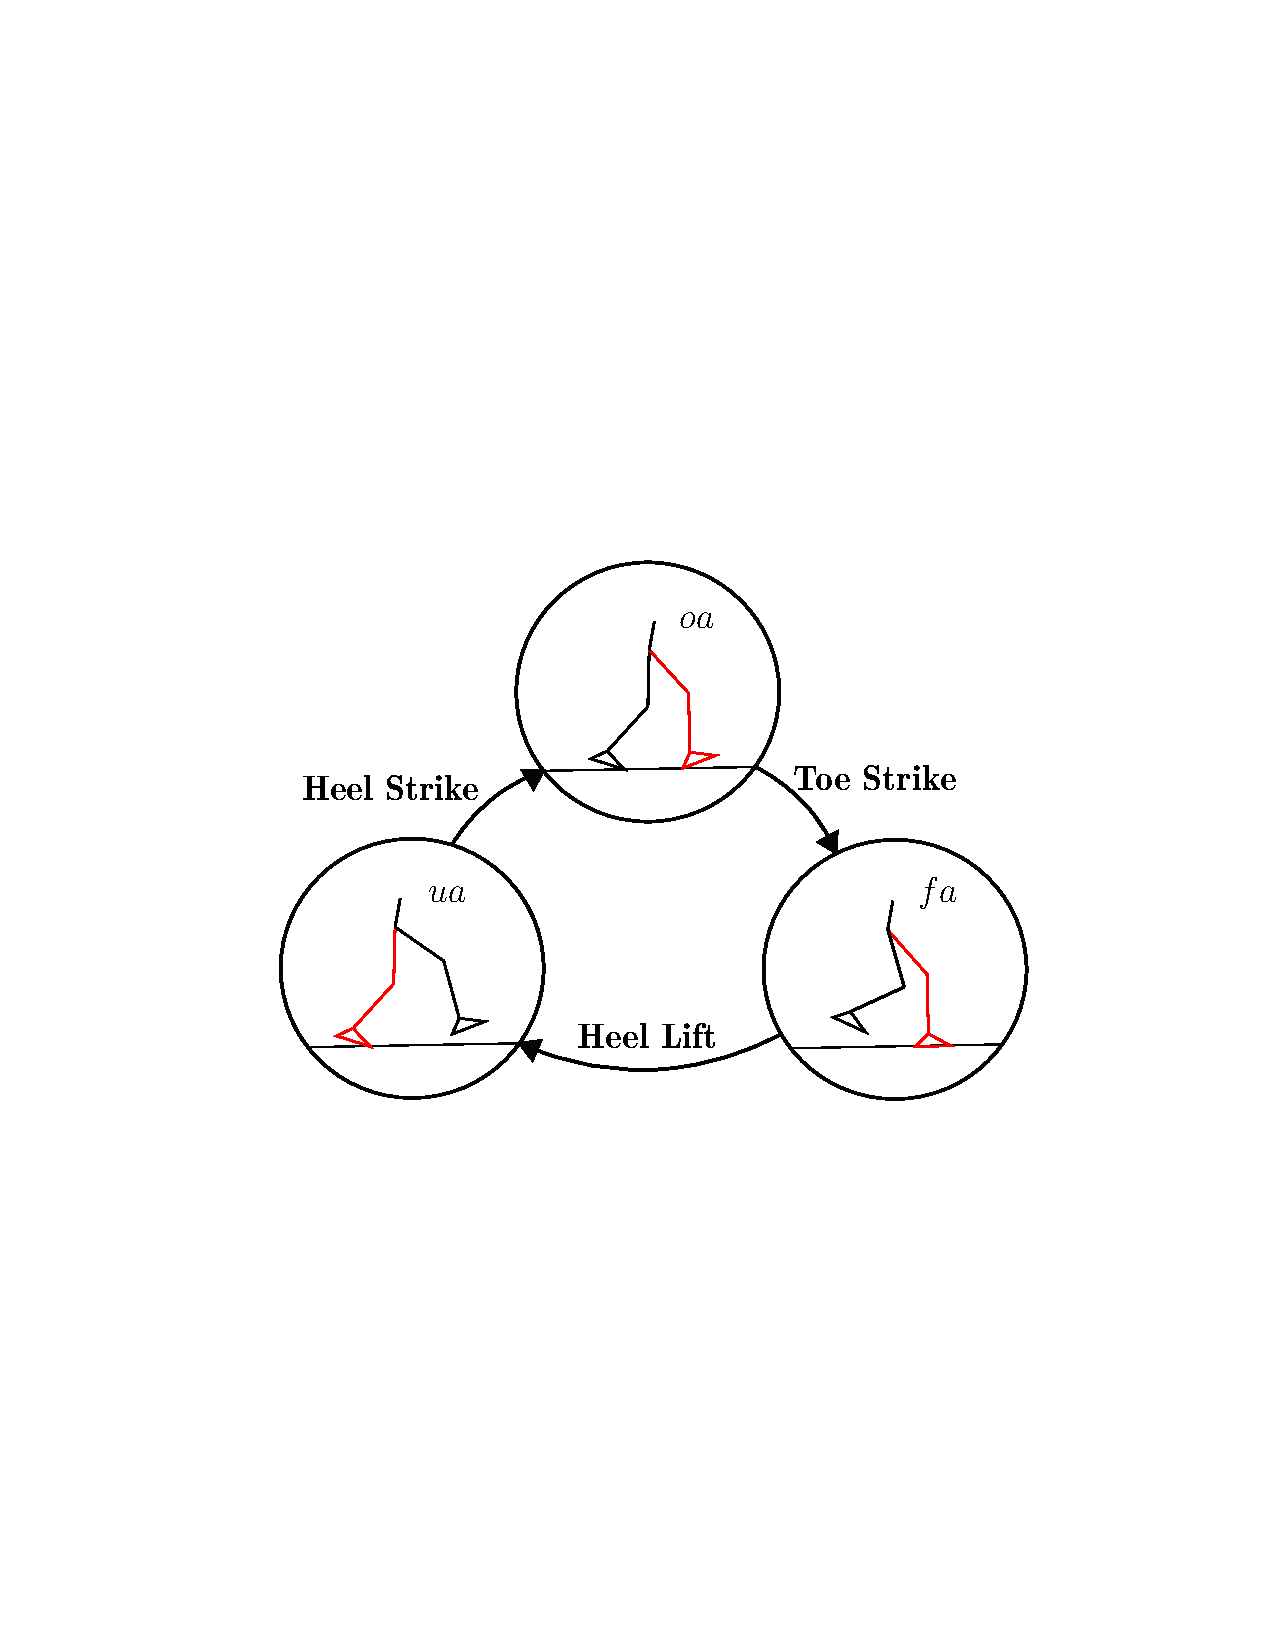
\includegraphics[width=0.35\textwidth]{figures/DomainGraph.pdf}
\caption{Directed graph associated with 3 domain walking. The red leg is the stance leg and the black leg is the non-stance leg.}
\label{fig:DomainGraph}
\end{figure}

\newsec{Hybrid System Model.}
The formal model of a bipedal robot with a multi-contact multi-domain walking gait follows the general development given in \cite{SPSA:IFAC:11}.  In particular, we consider a {\it hybrid control system model} given by a tuple:
 \begin{align}
 \label{eqn:HC}
  \HC = (\Gamma, \domain, \admissiblecontrol, \guard, \resetmap, \controlsystem),
 \end{align}
 where $\Gamma = (V,E)$ is a directed graph with vertices and edges,
  $D$ a set of domains, $U$ a set of admissible controls, $\Delta$ a set of reset maps, and $FG$ a control system. For a generalized definition of each element we refer the reader to \cite{SPSA:IFAC:11}.
The remainder of this section will be devoted to defining the specific elements of this hybrid system in the context of the multi-domain walking gait of interest. 

\newsec{Graph Structure.}  For the multi-contact walking gait of interest, the graph $\Gamma$ of the hybrid system $\HC$ is pictured in Fig. \ref{fig:DomainGraph}.   In particular, the discrete structure of the walking gait implies that $\Gamma$ is a directed cycle, with vertices and edges given by:
\begin{align}
 \VertexSet &= \{ \oa, \fa , \ua \}\\
 \EdgeSet   &= \{ \ts = (\ds \to \fa),\hl =(\fa \to \ua), \hs = (\ua \to \ds) \}.\nonumber
\end{align}
where in this case, we have labeled the vertices (also referred to as domains) by the type of actuation each of these domains display (as will be discussed later), i.e., the vertices $\oa$, $\fa$ and $\ua$ correspond to over, full and under actuation, respectively. 

\begin{figure}
\begin{subfigure}{0mm}
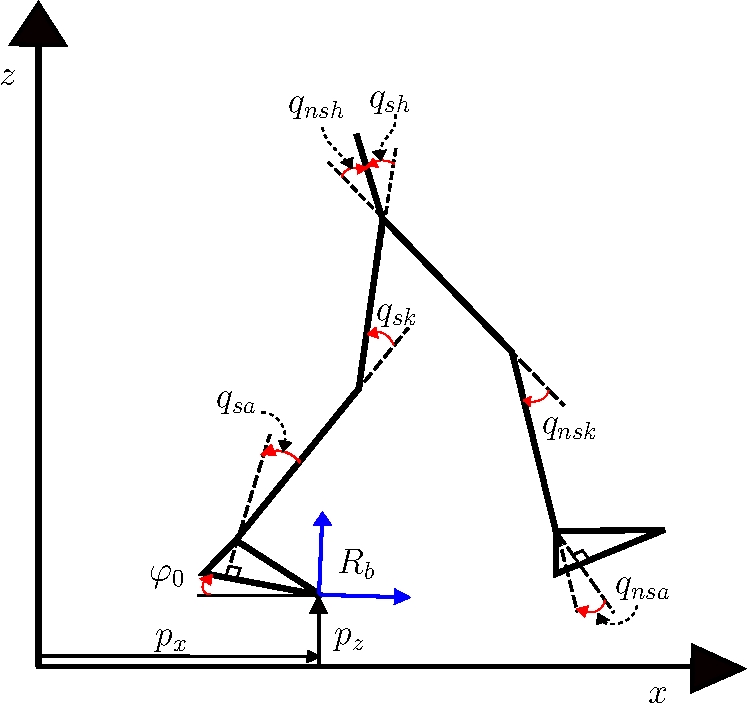
\includegraphics[width=40mm]{figures/RobotCoords.pdf}
\end{subfigure}
\hbox{\hspace{40mm}
\begin{subfigure}{0mm}
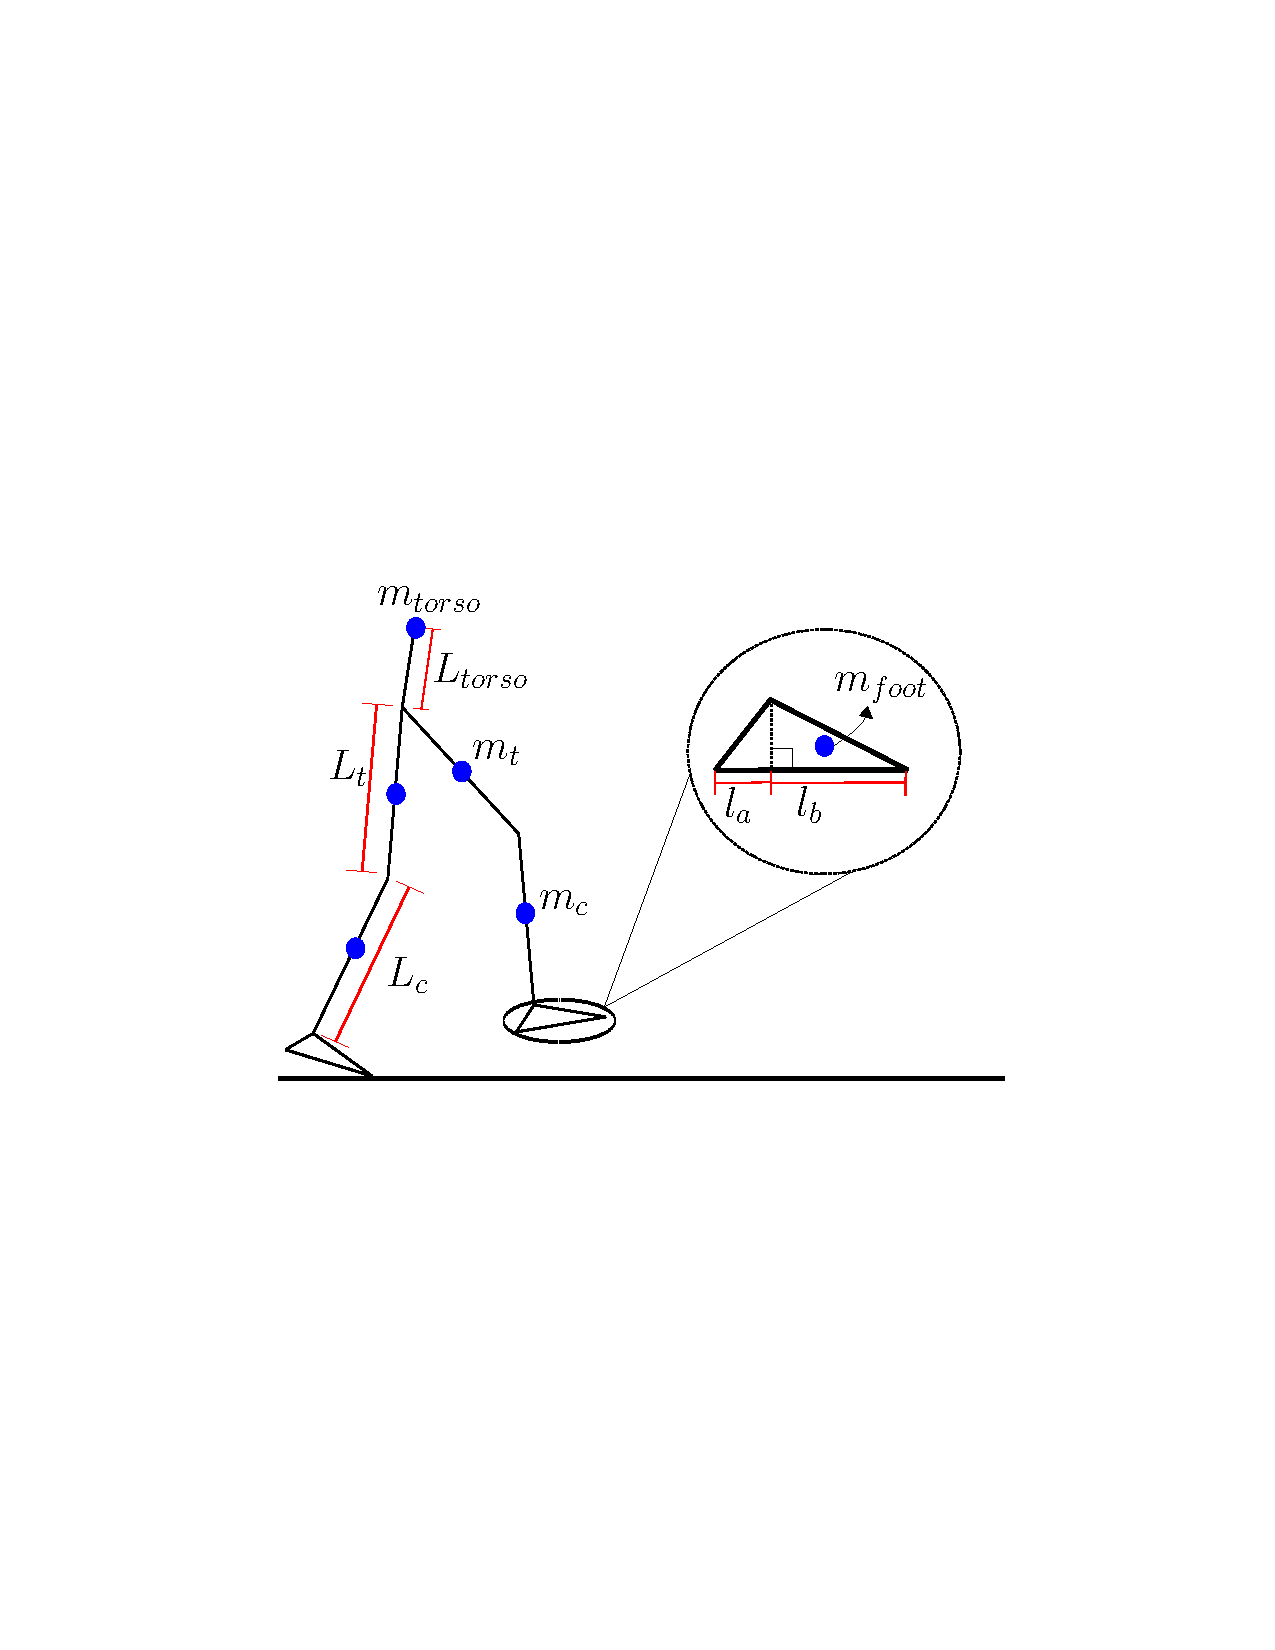
\includegraphics[width=50mm]{figures/RobotConfig.pdf}
\end{subfigure}}
\caption{Coordinates of 9 degree of freedom footed biped model (left) and layout of physical parameters (right).}
\label{fig:robotCoords}
\end{figure}


\newsec{Coordinates, Constraints and Actuation Types.}
We will now introduce basic terminology related to coordinates, constraints and actuation types that will be necessary to define the hybrid control system \eqref{eqn:HC} modeling a planar bipedal robot exhibiting a multi-domain walking gait. In particular, due to the multi-domain structure of the hybrid system model, this involves considering the generalized coordinates of the robot $Q = \mathbb{R}^{2} \times SO(2) \times Q_{r}$ where $Q_{r}$ is characterized by the relative joint angles(see Fig \ref{fig:robotCoords}). Specifically, $q = \{p_{x},p_{z},\varphi_{0},q_{r}\}$ where $q_{r} = \{q_{sa},q_{sk},q_{sh},q_{nsh},q_{nsk},q_{nsa}\}$ and $\{p_{x},p_{z},\varphi_{0}\}$ reference the body fixed frame $R_{b}$ with respect to a fixed inertial frame $R_{0}$ shown in Fig. \ref{fig:robotCoords}.
% : $Q = \Reals^2 \times SO(2) \times Q_r$, where $Q_r$ is the (relative) configuration space of the robot characterized by the relative angles of the system.  We assume that a subset of $Q_r$ are chosen so that there is a well-defined coordinate system, i.e., so that $Q_r$ is embeddable in $\Reals^{n_r}$, $Q_r \subset \Reals^{n_r}$, with coordinates expressed as $q_r \in Q_r$.  The generalized coordinate space $Q \subset \Reals^{n}$,  can be expressed in coordinates as $q = (p^T,\varphi_{0},q_r)^T$, where $p = (p^x,p^y)^T$ is a point and $\varphi_{0} \in SO(2)$ is an angle expressing the position and orientation of a reference frame, $R_b$, attached to the body of the robot relative to a world frame $R_0$.

% \gap

% \begin{myexample}
% For the simulation results presented in this paper (see Sec. \ref{sec:simresults}), the bipedal robot AMBER 2 will be considered; this robot can be seen in Fig. \ref{fig:robots}.  For this robot, the configuration space is given by $\indexbyrobot{\q} = \{ \qsa, \qsk, \qsh, \qnsh, \qnsk, \qnsa\}$, with the specific joint angles shown in Fig. \ref{fig:robotCoords}. 
% \end{myexample}

% \gap

{\it Contact Conditions:}  For each vertex of the graph $\Gamma$, there are associated contact points interacting with the physical world that dictate multi-contact conditions in the robot \cite{AVB:HSCC:11}. 
 This is represented by a set of contact points $\ContactSet = \{ sh, st, nsh, nst\}$, where $sh$ is the stance-heel, $st$ is the stance-toe, $nsh$ is the non-stance heel and $nst$ is the non-stance toe. With this, we consider two types of constraints: \emph{unilateral}, denoted $h_{v}$, and \emph{holonomic}, denoted $\eta_{v}$. Unilateral constraints dictate the set of admissible configurations, while holonomic constraints are used to encode which points are in contact with the walking surface.
 % indicating which points on the robot can, or are, interacting with the world.  Since we are considering a planar robot locomoting, we need only consider the contact points associated with the feet, i.e., $sh$ is the stance-heel, $st$ is the stance-toe, $nsh$ is the non-stance heel and $nst$ is the non-stance toe.  Associated with the indexing set of contact points are two types of constraints: {\it unilateral} and {\it holonomic}.   Unilateral constraints, denoted by $h_v$ for $v \in V$, are a vector-valued function that dictates the admissible configurations of the system on each domain by codifying which contact points are not on the ground, and therefore must stay above the ground for the current contact configuration to hold true.  Conversely, holonomic constraints, denoted by $\eta_v$ for $v\in V$, is a vector-valued function encoding which contact points are in contact with the ground and, therefore, must be held constant. 

\begin{myexample}
To provide a specific example, for the domain structure considered in this paper (see Fig. \ref{fig:DomainGraph}) there are the following constraints for each domain:
 \begin{itemize}
 \item For $v = \fa \in V$, $h_{\fa}(q)$ is the vertical reaction force at the stance heel, and $\eta_{\fa}(q)$ consists of the $x$, $z$ position of the stance toe together with the $z$ position of the stance heel.
\item For $v = \ua \in V$, $h_{\ua}(q)$ consists of the $z$ position of the non-stance heel, while $\eta_{\ua}(q)$ consists of the $x$, $z$ position of the stance toe.
\item For $v = \oa \in V$, $h_{\oa}(q)$ consists of the $z$ position of the stance toe, while $\eta_{\oa}(q)$ consists of the $x$, $z$ position the stance heel and the $z$ position of the stance toe.
 \end{itemize}
\end{myexample}

\gap

{\it Actuation Type:}  With notions of coordinates and constraints in hand, we wish to make explicit what is meant by full, over and under actuation. Let $m_r$ denote the number of actuators of the robot, $n = 9$ the number of unconstrained degrees of freedom of the robot, and $n_{c_v}$ denote the number of holonomic constraints in a given domain $v \in V$.  We say that a domain, $v \in V$, is
\begin{itemize}
 \item {\it Fully-actuated} if  $m_r = n - n_{c_v}$,
 \item {\it Under-actuated} if $m_r < n - n_{c_v}$,
 \item {\it Over-actuated} if  $m_r > n - n_{c_v}$. 
\end{itemize}
Similarly, we define the $V_{fa}$ to be the set of full-actuated domains, $V_{ua}$ to be the set of under-actuated domains, and $V_{oa}$ to be the set of over-actuated domains. 

\gap

\begin{myexample}
AMBER 2 has six actuators, thus $m_{r} = 6$. For $\oa \in V$, $n_{c_{\oa}} = 4$ thus $n - n_{c_{\oa}} = 9 - 4 = 5 < 6$ and the robot is over-actuated in $\oa$. For $\fa$, $n_{c_{\fa}} =3$ thus $n - n_{c_{\fa}} = 9 - 3 = 6$ and therefore the robot is said to be fully-actuated in $\fa$. For $\ua$, $n_{c_{\ua}}=2$ thus $n - n_{c_{\ua}} = 9 - 2 = 7>6$ and therefore the robot is under-actuated in $ua$. Note that it is useful to refer to this example when reading Section \ref{sec:control}.
\end{myexample}


\newsec{Continuous Dynamics.}
 We now have the necessary framework in which to construct the control system 
 \begin{align}
 \label{eqn:fgdyn}
 \xdot = \indexbyvertex{f}(\x) + \indexbyvertex{g}(\x) \control, \qquad v \in V
 \end{align}
 for each domain of the hybrid system $\HC$ given in \eqref{eqn:HC} where $x = (q,\dot{q})$.  In particular, the dynamics on each domain will be obtained from general ``unpinned'' dynamics through the use of holonomic constraints.

We begin by considering the unconstrained dynamics of the robot, i.e., the ``unpinned'' dynamics of the robot obtained by assuming no contact with the environment. Holonomic constraints are then used to enforce contact conditions. For a detailed derivation of the constrained dynamics we refer the reader to \cite{GCAS10}. The resulting constrained dynamical system is described by,
% \begin{align}
%  \nonumber
%  \Lagrangian(\q,\dq) = \frac{1}{2} \dq^T M(q) \dq  - \PotentialEnergy(\q), 
% \end{align}
% with $\GeneralizedInertia$ the generalized inertia matrix.  The Euler-Lagrange equations yield the equations of motion, which for robotic systems \cite{MLS94} are of the form:
% \begin{align}
%  \label{eq_eulerlagrange}
%  \GeneralizedInertia\ddq + \CoriolisGravity = \TorqueDistribution \control,
% \end{align}
% where $\CoriolisGravity = \Coriolis + \Gravity$ contains the Coriolis and gravity effects, $\TorqueDistribution$ is the torque distribution matrix, and $\control$ is the vector of actuator torques.
% Recall that for a domain $\vertex \in \VertexSet$, the holonomic constraints that are imposed on that domain are given by $\indexbyvertex{\holonomic}(\q)$.  Differentiating the holonomic constraints yields the constraint:
% \begin{align}
% \label{eqn:JT}
%  \indexbyvertex{\Jacobian}(\q) \dq = 0,
% \end{align}
% where $\indexbyvertex{\Jacobian}(\q) = \text{RowBasis} (\frac{\partial \indexbyvertex{\holonomic}(\q)}{\partial \q})$ is a basis for the row space of the Jacobian (this removes any redundant constraints so that $\indexbyvertex{\Jacobian}$ has full row rank). The constraint \eqref{eqn:JT} yields the \textit{constrained dynamics} on each domain $v \in V$:
\begin{align}
 \GeneralizedInertia\ddq + C(q,\dot{q})\dot{q} + G(q) = \TorqueDistribution \control + \indexbyvertex{\Jacobian}(q)^T \indexbyvertex{\ContactWrench}
 \label{eq_eulerlagrangeconstrained}
\end{align}
which enforces the holonomic constraint; here $\GeneralizedInertia$, $C(q,\dot{q})$ and $G(q)$ are the inertia matrix, coriolis matrix, and gravity vector and $\indexbyvertex{\ContactWrench}$ is the \textit{wrench} containing forces and moments expressed in the reference frame body frame \cite{GCAS10}. The constrained dynamics along with the holonomic constraints allows for the contact wrench to be solved for in terms of the state variables and joint torques(see \cite{GCAS10}).
% To determine the wrench $\indexbyvertex{\ContactWrench}$, we differentiate the kinematic constraint:
% \begin{align}
% \label{eqn:JJdotequaiton}
%  \indexbyvertex{\Jacobian}(q) \ddq + \dot{J}_v(q) \dq = 0,
% \end{align}
% and combine this equation with \eqref{eq_eulerlagrangeconstrained} to obtain an expression for $\indexbyvertex{\ContactWrench} (\q,\dq,\control)$ which is affine in $\control$. Therefore, by defining $\x = (\q^T, \dq^T)^T$, \eqref{eq_eulerlagrangeconstrained} and \eqref{eqn:JJdotequaiton} yields the affine control system of the form \eqref{eqn:fgdyn}. 

\newsec{Discrete Dynamics.} We now construct the continuous domains, $D$, guards, $S$, and reset maps $\Delta$, for a hybrid system \eqref{eqn:HC} using the unilateral and holonomic constraints.

Given a vertex $\vertex \in \VertexSet$, the continuous domain is the set of admissible configurations of the system factoring in both friction and a unilateral constraint. Specifically, from the wrench $\indexbyvertex{\ContactWrench} (\q,\dq,\control)$, one can ensure that the foot does not slip by considering inequalities on the friction which can be stated in the form: $\indexbyvertex{\frictioncoefficient}(q)^T \indexbyvertex{\ContactWrench}(\q,\dq,\control) \geq 0$, with $\indexbyvertex{\frictioncoefficient}$ a matrix of friction parameters (see \cite{SPSA:IFAC:11} for more details). These are coupled with the unilateral constraint on this domain, $\indexbyvertex{\unilateral}(q)$, to yield the set of admissible configurations:
\begin{align}
\indexbyvertex{\ConstraintMatrix}(\q,\dq,\control) &= \left[
  \begin{array}{c}
    \indexbyvertex{\frictioncoefficient}(q)^T \indexbyvertex{\ContactWrench}(\q,\dq,\control) \\
    \indexbyvertex{\unilateral}(q)
  \end{array}
  \right] \geq 0.
\end{align}
The continuous domain is thus given by:
\begin{align}
 \indexbyvertex{\domain} = \{ (\q,\dq,\control) \in TQ \times \Reals^{\indexbyvertex{\dimensionu}} : \indexbyvertex{\ConstraintMatrix}(\q,\dq,\control) \geq 0 \}.
\end{align}
The guard is just the boundary of this domain with the additional assumption that the set of admissible configurations is decreasing, i.e. the vector field is pointed outside of the domain, or for an edge $\edge =(\vertex \to \vertex') \in \EdgeSet$,
\begin{align}
 \indexbyedge{\guard} = \{ (\q,\dq,\control) \in TQ \times \Reals^{\indexbyvertex{\dimensionu}} : h_{v} = 0 \hspace{1mm} \\
  \nonumber \text{and} \hspace{1mm} \dot{h}_{v} < 0\}.
\end{align}
%\begin{align}
% \indexbyedge{\guard} = \{ (\q,\dq,\control) \in TQ \times \Reals^{\indexbyvertex{\dimensionu}} : \indexbyvertex{\ConstraintMatrix}(\q,\dq,\control) = 0 \hspace{1mm} \\
%  \nonumber \text{and} \hspace{1mm} \indexbyvertex{\dot \ConstraintMatrix}(\q,\dq,\control) < 0\}.
%\end{align}
The impact equations are given by considering the holonomic constraints enforced on the subsequent domain.  In particular, the post-impact velocity $\dq^+$ is given in terms of the pre-impact velocity $\dq^-$. With this, the reset map\footnote{Note that as a result of considering ``stance'' and ``non-stance'' legs, the labeling on the legs must be switching during one of the transitions; in this paper, these switching occurs at heel strike.  This is a common ``trick'' in robotic walking used to reduce the number of discrete domains.} is given by,
% \begin{align}
%  \dq^+ & = \indexbyedge{P}(\q, \dq^-)  \\
%    & = (I - \GeneralizedInertia^{-1} \Jacobian_{\vertex'}^T (\Jacobian_{\vertex'} \GeneralizedInertia^{-1} \Jacobian_{\vertex'}^T)^{-1} \Jacobian_{\vertex'}) \dq^-
% \end{align}
\begin{align}
 \indexbyedge{\resetmap}(\q,\dq) = \left[
    \begin{array}{c}
      \q \\
      \indexbyedge{P}(\q,\dq)
    \end{array}
    \right]
\end{align}
where $P_{e}$ is computed from the impact equations assuming perfectly plastic impacts(see \cite{WGCCM07}). The end result is that the hybrid model for the biped of a 2D bipedal robot is now completely defined.


\section{Multi-Domain Human-Inspired Control}
\label{sec:control}

This section extends the framework of human-inspired control \cite{Ames11} to the multi-contact case, i.e., 
the case where there are multiple discrete domains.  In particular, it is necessary to consider phases of under, over and full actuation.  
This general construction, applicable to general mixed actuation gaits, will be specialized the case of AMBER 2 
for the discrete structure given in Fig. \ref{fig:DomainGraph}.  



%elaborates on the general human-inspired control approach for bipedal robotic locomotion REFERENCE followed by specific examples of controller and hybrid system construction for the AMBER2, three-domain cycle of interest.

Consider the following system defined on each domain $v \in V$:
\begin{align}
\xdot &= \indexbyvertex{f}(\x) + \indexbyvertex{g} (\x) \control,\\
\indexbyvertex{\controloutput} &= \indexbyvertex{\controloutput^a}(x) - \indexbyvertex{\controloutput^d}(x),
\end{align}
for $\x \in \indexbyvertex{\domain}$ and $\control \in \indexbyvertex{\admissiblecontrol}$ and where $\indexbyvertex{\controloutput} $ is a \textit{control output} for $\vertex \in \VertexSet$, consisting of the difference between an actual output $\indexbyvertex{\controloutput^a}(x)$ and a desired value for this output $\indexbyvertex{\controloutput^d}(x)$. The human-inspired control design process consists of proper choice of actual and desired outputs, along with construction of a control law $u(\q,\dq)$ that drives $\indexbyvertex{\controloutput^a}(x) \to \indexbyvertex{\controloutput^d}(x)$ such that the resulting hybrid system obtained by applying this control law has a periodic orbit, i.e., a walking gait. 

\newsec{Human Locomotion (Actual) Outputs.}
Motivated by the consideration of human locomotion data in previous work \cite{AVB:HSCC:11}, we will construct the actual outputs, $\indexbyvertex{\controloutput^a}$, through the use of human output combinations \cite{Ames:TAC:2012}. 

\begin{mydefinition}
A human output combination for $\vertex \in \VertexSet$ is a tuple $\indexbyhuman{\humanoutputcombo} = (\indexbyrobot{\ConfigurationSpace},\indexbyhuman{\yone},\indexbyhuman{\ytwo})$ consisting of a configuration space $\indexbyrobot{\ConfigurationSpace}$, a velocity-modulating output $\indexbyhuman{\yone} : \indexbyrobot{\ConfigurationSpace} \to \Reals$ and position-modulating outputs $\indexbyhuman{\ytwo} : \indexbyrobot{\ConfigurationSpace} \to \Reals^{\dimensionx-1}$. Let $\OutputSet_v$ be an indexing set for $\indexbyhuman{\ytwo}$ whereby $\indexbyhuman{\ytwo}(\q) = [\indexbyhuman{\ytwo}(\q)_\youtput]_{\youtput \in \OutputSet_v}$. A set of human outputs are \textit{independent} if,
 \begin{align}
  \text{rank}( \left[
    \begin{array}{c} \indexbyhuman{\yone}(\q,\dq) \\
                     \indexbyhuman{\ytwo}(\q)
    \end{array}
    \right]) = \indexbyvertex{\dimensionx},
 \end{align}
on $\indexbyrobot{\ConfigurationSpace}$, and \textit{linear} if
\begin{align}
 \indexbyhuman{\yone}(\q) &= \indexbyvertex{\dyonedq} \q \\
 \indexbyhuman{\ytwo}(\q) &= \indexbyvertex{\dytwodq} \q
\end{align}
for $\indexbyvertex{\dyonedq} \in \Reals^{1 \times \indexbyvertex{\dimensionx}}$ and $\indexbyvertex{\dytwodq} \in \Reals^{(\indexbyvertex{\dimensionx}-1) \times \indexbyvertex{\dimensionx}}$.
\end{mydefinition}

\gap

\begin{myexample}
 We choose the following linear and independent human output combinations for the three domains of interest. For the velocity modulating output, we consider the same linear output for all three domains characterized by:
 \begin{eqnarray}
  \dyonedq_{v} = \left[ \begin{array}{c c c c c c c c c}
  0 &0 &0 & -\lengthofcalf -\lengthofthigh & -\lengthofthigh& 0 & 0 & 0 & 0
 \end{array}\right] 
 \end{eqnarray}
 for $v \in V = \{\ds,\fa,\ua\}$, with $\lengthofcalf$ the length of the calf and $\lengthofthigh$ the length of the thigh of the robot.   For the position modulating outputs, we first consider the linear outputs for the under-actuated domain characterized by
  \begin{align}
  \dytwodq_{\ua} &= \left[ \begin{array}{c c c c c c c c c}
  0 &0 &0 & 1 & 0 & 0 & 0 & 0 & 0  \\
  0 &0 &0 & 0 & 1 & 0 & 0 & 0 & 0  \\
  0 &0 &0 & 0 & 0 & 0 & 0 & 1 & 0\\
  0 &0 &0 & 0 & 0 & 1 & -1 & 0 & 0\\
  0 &0 &1 & 1 & 1 & 1 & 0 & 0 & 0\\
  0 &0 &1 & 1 & 1 & 1 & -1 & -1 & -1\\
 \end{array}\right]
 \end{align}
 The position modulating outputs for the over- and fully-actuated domains are chosen to be submatrices of $\dytwodq_{\ua}$ based upon the available degrees of actuation in these respective domains.  In particular, $\dytwodq_{\ds} = (\dytwodq_{\ua})_{1,2,5,6}$ and  $\dytwodq_{\fa} = (\dytwodq_{\ua})_{2-6}$, where here we have used the notation $(\dytwodq_{\ua})_{i}$ to denote the $i^{\mathrm{th}}$ row of $\dytwodq_{\ua}$.
Note that this is not the only valid choice of human output combination, but the one chosen here based upon examination of human locomotion data.
\end{myexample}


\newsec{Canonical Walking Functions.} Previous results \cite{ZYA2012,AVB:HSCC:11,PZA2012} reveal that for the actual outputs considered, humans tend to display very simple behavior.  This observation motivates the use of simple desired functions for bipedal locomotion. In particular, it was observed \cite{AVB:HSCC:11} through examination of human walking data that the for ``proper'' choices of the velocity modulating output---as calculated from human walking data---satisfies the property that:
\begin{align}
\label{eqn:y1approx}
  \indexbyhuman{\yone}(\q) \approx \vhip t
\end{align}
 In addition, by selectively choosing the human outputs, they appear to be described by the solution to a linear mass-spring damper system. With this in mind, define the \textit{canonical walking function}:
\begin{align}
 \controloutput_{\cwf} (t, \param) = e^{-\param_4 t} (\param_1 \cos( \param_2 t) + \param_3 \sin(\param_2 t) ) + \param_5
\end{align}
Additionally, it was found that for more complex walking behavior, e.g., stair climbing and rough terrain locomotion \cite{PZA2012,SA:SSRR:2012}, the position modulating outputs appear to be described by the solution to a linear mass-spring-damper system under sinusoidal excitation. With this in mind, define the \textit{extended canonical walking function}:
\begin{align}
\nonumber
 \controloutput_{\ecwf} (t, \param) = &e^{-\param_4 t} (\param_1 \cos( \param_2 t) + \param_3 \sin(\param_2 t) ) \\
 &+ \param_5 \cos(\param_6 t) + \kappa(\param) \sin(\param_6 t) + \param_7,
\end{align}
where $\kappa(\param) = (2\param_4\param_5\param_6)/((\param_2)^2+(\param_4)^2+(\param_6)^2)$. As found in \cite{Ames11} these functions represent (human) bipedal locomotion data with high correlation and therefore, we leverage these functions in construction of desired control outputs for bipedal locomotion and claim that the functions are natural suggestions for bipedal (human and robotic) walking.

\newsec{Parameterization of Time.} 
With these time-based functions in mind, and specifically \eqref{eqn:y1approx}, coupled with the desire to construct \textit{autonomous} control functions, that is, functions which are independent of time, we specify the following \textit{parameterization of time}:
\begin{align}
 \indexbyvertex{\timeparameterization}(\q) = \frac{\indexbyhuman{\yone}(\q)-\pzero}{\vhip}
\end{align}
where $\pzero \in \Reals$ is used to align $\indexbyvertex{\timeparameterization}(\q)=0$ at critical points in the gait, i.e. at the start of specific domains $\vertex \in \VertexSet$.  

%, for which we make the substitution $t \to \indexbyvertex{\timeparameterization}(\q)$ in EQREF and EQREF. We seek an autonomous control law, through this parameterization, for increased robustness.

\newsec{Desired Output functions.} Based upon the human outputs and their time-based representation given by the canonical walking functions, we define outputs for the robot based upon our desire for the robot to have the same output behavior as a human. With the goal of controlling the forward velocity of the robot, we define the relative degree one desired output to be:
\begin{align}
 \ydone = \vhip, \qquad v \in V
\end{align}
for all domains, i.e., irrespective of actuation type.  Similarly, with the goal of the robot tracking the canonical walking function, for the over actuated domains, we define the desired outputs to be:
\begin{align}
 \ydtwo(\indexbyvertex{\timeparameterization}(\q),\indexbyvertex{\param}) = [y_{cwf}(\indexbyvertex{\timeparameterization}(\q),\indexbyvertex{\param}^i)]_{i \in \OutputSet_v}, \:\: v \in V_{oa}
\end{align}
that is, for $v \in  V \:\: \mathrm{s.t} \:\: m_r > n - c_v$.  Finally, in the case of either fully or under actuation, we define the desired output to be:
\begin{align}
 \ydtwo(\indexbyvertex{\timeparameterization}(\q),\indexbyvertex{\param}) = [y_{ecwf}(\indexbyvertex{\timeparameterization}(\q),\indexbyvertex{\param}^i)]_{i \in \OutputSet_v}, \:\: v \in V_{fa} \cup V_{ua}
\end{align}
that is, for $v \in V \:\: \mathrm{s.t} \:\: m_r \leq n - c_v$. 
%
%
%we consider the following relative degree two outputs for $v = ds$, i.e. in the double support domain:
%\begin{align}
% \ydtwo(\indexbyvertex{\timeparameterization}(\q),\indexbyvertex{\param}) = [y_{cwf}(\indexbyvertex{\timeparameterization}(\q),\indexbyvertex{\param}^i)]_{i \in \OutputSet}.
%\end{align}
%Similarly, with the goal of the robot tracking the canonical walking function, we consider the following relative degree two outputs for $v = fa$ and $v=ua$, i.e. in the fullyactuated and underactuated domains:
%\begin{align}
% \ydtwo(\indexbyvertex{\timeparameterization}(\q),\indexbyvertex{\param}) = [y_{ecwf}(\indexbyvertex{\timeparameterization}(\q),\indexbyvertex{\param}^i)]_{i \in \OutputSet}.
%\end{align}

\newsec{Control Law Construction.} The goal is to drive the outputs of the robot, obtained through a human output combination, to the outputs of the human as represented by the canonical walking functions parameterized by $\indexbyvertex{\timeparameterization}(\q)$. This motivates the final form of the outputs, termed the \textit{human-inspired outputs} and given by, for all $v \in V$:
\begin{align}
 \yone(\q,\dq) &= \frac{\partial y^H_{1,v} (q)}{\partial \q} \dq -\vhip\\
 \ytwo(\q) &= y^H_{2,v}(\q) - \ydtwo(\indexbyvertex{\timeparameterization}(\q), \indexbyvertex{\param})
\end{align}

%Since the type of actuation of the robot is determined by the interplay between the generalized coordinates and the constraints enforced on a given domain, we can define a controller for all $v \in V$ for which only the output vectors that define this controller change.  That is, we can define the \textit{multi-domain human-inspired controller} by:

From these outputs, we can construct two types of controllers: one for the fully and over actuated domains, and one for the under actuated domain.  In the case of full and over actuation, we define the {\it human-inspired controller} by:
\begin{align}
\label{eqn:uv}
 \indexbyvertex{\control^{(\param_{v},\controlgain)}}(\q,\dq)& = -\indexbyvertex{\decouplingmatrix}^{-1}(\q,\dq)  \left( \left[ \begin{array}{c} 0 \\ L_{f_v}L_{f_v}\ytwo(\q, \dq) \end{array} \right]\right.  \\ &+ \left.\left[ \begin{array}{c} L_{f_v}\yone(\q, \dq) \\ 2 \controlgain L_{f_v}\ytwo(\q, \dq) \end{array} \right] + \left[ \begin{array}{c} \controlgain \yone(\q,\dq) \\ \controlgain^2 \ytwo(\q) \end{array} \right] \right),
 \nonumber
\end{align}
for $v \in V_{fa} \cap V_{oa}$.  Here $L$ is the Lie derivative, $\controlgain > 0$ is a user defined control gain that dictates the convergence of $\yone$ and $\ytwo$ to 0, and
\begin{align}
 \indexbyvertex{\decouplingmatrix}(\q,\dq) = \left[ \begin{array}{c} L_{g_v}\yone(\q, \dq) \\ L_{g_v}L_{f_v}\ytwo(\q, \dq) \end{array} \right].
\end{align}
is the decoupling matrix.  In a similar fashion, in the case of underactuation, we define the human-inspired controller:  
\begin{align}
\label{eqn:uvunder}
 \indexbyvertex{\control^{(\param_{v},\controlgain)}}(\q,\dq) = -&\indexbyvertex{\decouplingmatrix}^{-1}(\q,\dq) \left( L_{f_v}L_{f_v}\ytwo(\q,\dq) + \right. \\
 & \left. 2 \controlgain L_{f_v}\ytwo(\q,\dq) + \controlgain^2 \ytwo(\q)\right) \nonumber
\end{align}
for $v \in \Vua$, where in this case $\decouplingmatrix =  L_{g_v}L_{f_v}\ytwo(\q, \dq)$.  We note that $\decouplingmatrix$ is assumed to non-singular for all $v \in V$ as a necessary condition for the human output combination $Y^H_v$ to be valid; this also implies that $\yone$ and $\ytwo$ have the proper (vector) relative degree.   Importantly, depending on the choice of outputs and constraints enforced, the control law \eqref{eqn:uv} is a controller for the case of under, full and over actuation.


Applying the feedback control law in \eqref{eqn:uv} and \eqref{eqn:uvunder} to \eqref{eqn:fgdyn} yields dynamical systems for each domain.   It is the behavior of this closed form system that we wish to analyze.  In particular, the goal is to find parameters $\param_{v}$ for each domain such that a hybrid periodic orbit is generated for the closed form system.  This is the aim of the human-inspired optimization problem that will be presented in the next section.

%This, in turn, yields a hybrid control system he hybrid control system modeling the bipedal robot being considered, yields a hybrid system.
%
%
%The feedback linearization controller for doublesupport, denoted by $\indexbydoublesupport{\control^{(\param_{ds},\controlgain)}}(\q,\dq)$ and termed the \textit{human-inspired controller} for double support due to its dependence on the human-inspired outputs, can now be stated as:
%\begin{align}
% \indexbydoublesupport{\control^{(\param_{ds},\controlgain)}}(\q,\dq)& = -\indexbydoublesupport{\decouplingmatrix}^{-1}(\q,\dq)  \left( \left[ \begin{array}{c} 0 \\ L_{f_r}L_{f_r}\ytwods(\q, \dq) \end{array} \right]\right.  \\ &+ \left.\left[ \begin{array}{c} L_{f_r}\yoneds(\q, \dq) \\ 2 \controlgain L_{f_r}\ytwods(\q, \dq) \end{array} \right] + \left[ \begin{array}{c} \controlgain \yoneds(\q,\dq) \\ \controlgain^2 \ytwods(\q) \end{array} \right] \right),
% \nonumber
%\end{align}
%with control gain $\controlgain$ and decoupling matrix
%\begin{align}
% \indexbydoublesupport{\decouplingmatrix}(\q,\dq) = \left[ \begin{array}{c} L_{g_r}\yoneds(\q, \dq) \\ L_{g_r}L_{f_r}\ytwods(\q, \dq) \end{array} \right].
%\end{align}
%Note that the decoupling matrix is non-singular by the definition of an admissible output combination see DEFINITION. More generally, this follows from the fact that care was taken when defining human output combinations so that the are independent see DEFINITION.
%
%Applying the feedback control law in EQREF to the hybrid control system modeling the bipedal robot being considered, yields a hybrid system.
%
%The feedback linearization controller for full actuation, denoted by $\indexbyfullactuation{\control^{(\indexbyvertex{\param},\controlgain)}}(\q,\dq)$ and termed the \textit{human-inspired controller} for full actuation due to its dependence on the human-inspired outputs, can now be stated as:
%\begin{align}
%\nonumber
% \indexbyfullactuation{\control^{(\param_{fa},\controlgain)}}(\q,\dq)& = -\indexbyfullactuation{\decouplingmatrix}^{-1}(\q,\dq)  \left( \left[ \begin{array}{c} 0 \\ L_{f_r}L_{f_r}\ytwofa(\q,\dq) \end{array} \right]\right.  \\ &+ \left.\left[ \begin{array}{c} L_{f_r}\yonefa(\q, \dq) \\ 2 \controlgain L_{f_r}\ytwofa(\q) \end{array} \right] + \left[ \begin{array}{c} \controlgain \yonefa(\q,\dq) \\ \controlgain^2 \ytwofa(\q) \end{array} \right] \right),
% \nonumber
%\end{align}
%with control gain $\controlgain$ and decoupling matrix
%\begin{align}
% \indexbyfullactuation{\decouplingmatrix}(\q,\dq) = \left[ \begin{array}{c} L_{g_r}\yonefa(\q, \dq) \\ L_{g_r}L_{f_r}\ytwofa(\q, \dq) \end{array} \right].
%\end{align}
%Note that the decoupling matrix is non-singular by the definition of an admissible output combination see DEFINITION. More generally, this follows from the fact that care was taken when defining human output combinations so that the are independent see DEFINITION.
%
%Applying the feedback control law in EQREF to the hybrid control system modeling the bipedal robot being considered, yields a hybrid system.
%
%\newsec{Underactuated Control.} When the robot is underactuated, there is no longer the control authority to drive all of the outputs of the system to be in agreement with the human outputs. In particular, since we will no longer have control of the stance ankle (as in the case of AMBER, due to its point feet), we can no longer directly control the forward movement of the hip through the output HUH. Thus, in the case of underactuation, we only consider the relative degree 2 outputs given in EQREF.
%
%Motivated by these considerations related to underactuated control, for the affine control system FGU associated with the robotic model EQREF, we define the \textit{human-inspired controller} for underactuation:
%\begin{align}
% \indexbyunderactuation{\control^{(\param_{ua},\controlgain)}}(\q,\dq) = -&\indexbyunderactuation{\decouplingmatrix}^{-1}(\q,\dq) \left( L_{f_r}L_{f_r}\ytwoua(\q,\dq) + \right. \\
% & \left. 2 \controlgain L_{f_r}\ytwoua(\q,\dq) + \controlgain^2 \ytwoua(\q)\right)
%\end{align}
%with y2 as defined in EQREF and the underactuated decoupling matrix. As in the case of full actuation, the decoupling matrix is non-singular because of the choice of output functions and the fact that we assume admissibility of the outputs. In addition, the control law $\indexbyunderactuation{\control^{(\indexbyvertex{\param},\controlgain)}}(\q,\dq)$ results in dynamics on the outputs given by EQREF and therefore renders the relative degree two outputs, y2, exponentially stable. Due to the fact that the system is underactuated, the output y1 will no longer converge to 0. Thus the velocity of the hip cannot be directly controlled in the case of underactuation.
%
%Applying the feedback control law in EQREF to the hybrid control system modelin the bipedal robot being considered, yields a hybrid system.









\section{Optimization}
\label{sec:optimization}

This section presents the formulation of an optimization problem which yields controller parameters for the three domain gait of interest. The objective function of this optimization is a least squares fit of controller outputs to corresponding outputs computed on human locomotion data. More novel to this paper, however, is the construction of equality and inequality constraints that--when satisfied--yield periodic, three-domain walking. Previous results using partial hybrid zero dynamics are leveraged.  \textit{Motion Transitions} \cite{PHA2013} are used to compute the controller parameters for full actuation, $\alpha_{fa}$, and under actuation, $\alpha_{ua}$. State reconstruction on a partial hybrid zero dynamics surface \cite{WGK03} is used to compute various physical constraints on the controllers, e.g. torque and reaction force constraints.


\newsec{Partial Hybrid Zero Dynamics.}
Previous methods introduce the notion of \textit{partial hybrid zero dynamics} surface
\begin{align}
\label{PZD}
\mathcal{PZ}_{v,\alpha} = \{(q,\dot{q}) \in Q : y_{2}(q) = \mathbf{0}, \dot{y}_{2}(q,\dot{q}) = \mathbf{0}\}
\end{align}
which has properties that are useful for obtaining controllers for periodic walking, as described in the proceeding sections. In particular, on this surface, a low dimensional representation of the system is obtained by defining the zero dynamics coordinates for $v \in \{oa,fa\}$,
\begin{align}
\xi_{v,1} = \delta p_{hip}(q), \hspace{3mm}
\xi_{v,2} = c_{v}\dot{q}
\end{align}
The usefulness of this low dimensional representation will be demonstrated in the next section.

\newsec{Inverse Kinematics.} We use the method found in \cite{ACP:HSCC12}, to compute a point $\vartheta(\alpha_{oa}) \in Q_{r}$ on the guard from the underactuated phase to the double support phase, $S_{ua \to oa}$. We use the fact that on a partial hybrid zero dynamics surface $y^{a}_{2,v} = y^{d}_{2,v}$ and on $S_{ua \to oa}$, both the stance heel and the nonstance toe must be on the ground. The point is obtained by solving
\begin{eqnarray}
\label{eq:inverse}
\vartheta(\alpha_{oa}) = q \hspace{3mm} s.t. \hspace{5cm} \nonumber\\
\left[ \begin{array}{c}
y^{a}_{oa,2}(q) - y^{d}_{oa,2} (0,\alpha_{oa}) \\
h_{oa}(q)
\end{array}
\right] =
\left[ \begin{array}{c}
\zm_4 \\
0
\end{array}
\right],
\end{eqnarray}
where $\tau_{\alpha_{oa}} = 0$ at the beginning of the over actuated domain. Using $\vartheta(\alpha_{oa})$, we can explicitly solve for a point $(\vartheta, \dot{\vartheta}) \in \mathcal{PZ}_{\alpha_{oa}} \cap S_{oa}$.
%\textit{zero dynamics manifold}:
%\begin{align}
% \nonumber
%\ZeroDynamics_{\indexbyvertex{\param}} = \{(\q,\dq) \in \ConfigurationSpace :  \hspace{1mm} &\yone(\q,\dq) = 0, \\&
%\ytwo(\q) = \mathbf{0}, \ydottwo(\q,\dq) = \mathbf{0}\}
%\label{eq:ZD}
%\end{align}
%where $\yone(\q,\dq)$ and $\ytwo(\q,\dq)$ are a set of relative degree one and two outputs. The following is a Partial Zero Dynamics Surface
%\begin{align}
%\label{PZD}
%\PartialZeroDynamics_{\indexbyvertex{\param}} = \{(\q,\dq) \in \ConfigurationSpace : \ytwo(\q) = \mathbf{0}, \ydottwo(\q,\dq) = \mathbf{0}\}
%\end{align}
%This motivates the notion of a \textit{partial hybrid zero dynamics} on a cycle:
%\begin{align}
%\label{PZD}
%\forall \hspace{1mm} \edge \in \EdgeSet, \hspace{3mm} \indexbyedge{\resetmap} ( \indexbyedge{\guard} \cap \PartialZeroDynamics_{\param_\sore} ) \subset \PartialZeroDynamics_{\param_\tare}
%\end{align}

\newsec{PHZD State Reconstruction.}\label{sec:reconstruction} As claimed in \cite{ACP:HSCC12}, states on a partial hybrid zero dynamics surface can be obtained as functions of the linearized position of the hip. For $v \in \{V_{oa},V_{fa}\}$, the states of the system can obtained through PHZD reconstruction. It follows that by defining,
\begin{align}
\Phi(\xi_{v,1}) = 
\begin{bmatrix}
c_{v} \\
H_{v}
\end{bmatrix}^{-1}
\begin{bmatrix}
\xi_{v,1} \\
y^{d}_{v,2}
\end{bmatrix}
, \\
\Psi(\xi_{v,1}) = 
\begin{bmatrix}
c_{v} \\
H_{v}
\end{bmatrix}^{-1}
\begin{bmatrix}
1 \\
\frac{\partial y^{d}_{v,2}}{\partial \xi_{v,1}}
\end{bmatrix} \nonumber
\end{align}
the point $(\q, \dq) \in \mathcal{PZ}_{\param_{\vertex}}$ is found by $q  = \Phi(\xi_{v,1})$ and $\dq  = \dqreconstruction(\xi_{v,1})\xi_{v,2}$. The next section will show how motion transitions are used to compute controller parameters $\alpha_{fa}$ and $\alpha_{ua}$ in closed form.
\begin{comment}
Furthermore, this method can be used to compute states at \textit{any} value of $\xi_{1,\vertex}$;  in the proceeding sections we take advantage of this fact to specify values of $\xi_{1,\vertex}$ at 
which to transition from one domain to another. Let $\beta_1$ be a \textit{transition point} from 
the over actuated domain to the fully actuated domain, such that $(\qreconstruction(\beta_1)
,\dqreconstruction(\beta_1)) \in \guard_{oa \to fa}$ and likewise, let $\beta_2$ be a transition 
point from the fully actuated domain to the under actuated domain, such that $(\qreconstruction
(\beta_2),\dqreconstruction(\beta_2)) \in \guard_{fa \to ua}$.
\end{comment}

\newsec{Motion Transitions.} It was shown in \cite{PHA2013} that we can connect any two PHZD surfaces together with the ECWF to ensure that partial hybrid zero dynamics is maintained, i.e. there is a closed form expression for parameters of the ECWF that yield a PHZD surface connecting two other PHZD surfaces. Let $(\q_{\sore}, \dq_{\sore}) \in \mathcal{PZ}_{\param_{\sore}}$ and $(\q_{\tare}, \dq_{\tare}) \in \mathcal{PZ}_{\param_{{\tare}}}$ be points in two partial zero dynamics surfaces.
Denoting a set of controller parameters $\alpha$ for a set of ECWF's, leveraging the fact that the ECWF is linear in some of the controller parameters, it can be written as,
\begin{align}
\hspace{-2mm} y_{ecwf}(\alpha^{i},\tau) = Y_{ecwf}(\alpha^{i}_{2},\alpha^{i}_{4},\alpha^{i}_{6},\tau(\xi_{1},v_{hip},d))
\begin{bmatrix}
\alpha^{i}_{1} \\
\alpha^{i}_{3} \\
\alpha^{i}_{5} \\
\alpha^{i}_{7}
\end{bmatrix}
\end{align}
where,
\begin{align}
& Y_{ecwf}(\alpha^{i}_{2},\alpha^{i}_{4},\alpha^{i}_{6},\tau(q)) = \\
& \begin{bmatrix}
e^{-\alpha^{i}_{4}\tau(\xi_{1},v_{hip},d})cos(\alpha^{i}_{2}\tau(\xi_{1},v_{hip},d)) \\
e^{-\alpha^{i}_{4}\tau(\xi_{1},v_{hip},d})sin(\alpha^{i}_{2}\tau(\xi_{1},v_{hip},d)) \\
cos(\alpha^{i}_{6}\tau(\xi_{1},v_{hip},d))+\frac{2*\alpha^{i}_{4}\alpha^{i}_{6}}{(\alpha^{i}_{2})^{2}
+(\alpha^{i}_{4})^{2}-(\alpha^{i}_{6})^{2}} \\
1
\end{bmatrix}^{T} \nonumber
\end{align}
Using the states at the points to be connected to define,
\begin{align}
& y^{0}_{i,2} = y_{ecwf}(\tau(\xi_{1},v_{hip},d_{sor})\alpha^{i}) \\
& \dot{y}^{0}_{i,2} = \frac{d}{d\xi_{1}}y_{ecwf}(\tau(\xi_{1},v_{hip},d_{sor}),\alpha^{i})\Big|_{\xi_{1}=\xi^{0}_{1}} \\
& y^{f}_{i,2} = y_{ecwf}(\tau(\xi_{1},v_{hip},d_{tar}),\alpha^{i}) \\
& \dot{y}^{f}_{i,2} = \frac{d}{d\xi_{1}}y_{ecwf}(\tau(\xi_{1},v_{hip},d_{tar}),\alpha^{i})\Big|_{\xi_{1}=\xi^{f}_{1}},
\end{align}
where $\xi^{0}_{1}$ is the position of the hip at $q = q_{sor(e)}$ and $\xi^{f}_{1}$ the position of the hip at $q = q_{tar(e)}$, the controller parameters $\alpha_{1},\alpha_{3},\alpha_{5}$, and $\alpha_{7}$ that connect the source and target domains can be solved for,
\begin{align}
\begin{bmatrix}
\alpha^{i}_{1} \\
\alpha^{i}_{3} \\
\alpha^{i}_{5} \\
\alpha^{i}_{7}
\end{bmatrix}
=
\mathbb{Y}^{-1}
\begin{bmatrix}
y^{0}_{i,2} \\
\dot{y}^{0}_{i,2} \\
y^{f}_{i,2} \\
\dot{y}^{f}_{i,2}
\end{bmatrix}
\end{align}
where,
\begin{align}
 \mathbb{Y} = 
 \begin{bmatrix}
  Y_{ecwf}(\xi_{1},v_{hip},d_{sor},\alpha^{i}_{2},\alpha^{i}_{4},\alpha^{i}_{6}) \\
  \frac{d}{d\xi_{1}} Y_{ecwf}(\xi_{1},v_{hip},d_{sor},\alpha^{i}_{2},\alpha^{i}_{4},\alpha^{i}_{6})\Big|_{\xi_{1}=\xi^{0}_{1}} \\
  Y_{ecwf}(\xi_{1},v_{hip},d_{tar},\alpha^{i}_{2},\alpha^{i}_{4},\alpha^{i}_{6}) \\
  \frac{d}{d\xi_{1}} Y_{ecwf}(\xi_{1},v_{hip},d_{tar},\alpha^{i}_{2},\alpha^{i}_{4},\alpha^{i}_{6})\Big|_{\xi_{1}=\xi^{f}_{1}}
 \end{bmatrix}.
\end{align}
Note that the motion transition solves for $\alpha_{1},\alpha_{3},\alpha_{5}$, and $\alpha_{7}$, leaving $\alpha_{2},\alpha_{4}$ and $\alpha_{6}$ to be freely chosen as long as the chosen values satisfy $(\alpha^{i}_{2})^{2}+(\alpha^{i}_{4})^{2}-(\alpha^{i}_{6})^{2} \neq 0$ to prevent division 
by zero. For the purposes of this paper, the points $(q_{sor},\dot{q}_{sor})$ and $(q_{tar},\dot{q}_{tar})$ are 
obtained via the PHZD reconstruction at $((q,\dot{q}) \in \mathcal{PZ}_{oa}) \cap S_{oa \rightarrow fa}$ and $((q,\dot{q}) \in \mathcal{PZ}_{fa}) \cap S_{fa \rightarrow ua}$ to connect the outputs to the target $(\vartheta(\alpha_{oa}),\dot{\vartheta}(\alpha_{oa}))$ resulting in the controller parameters $\alpha_{fa}$ and $\alpha_{ua}$.
\begin{figure}[t!]
\centering
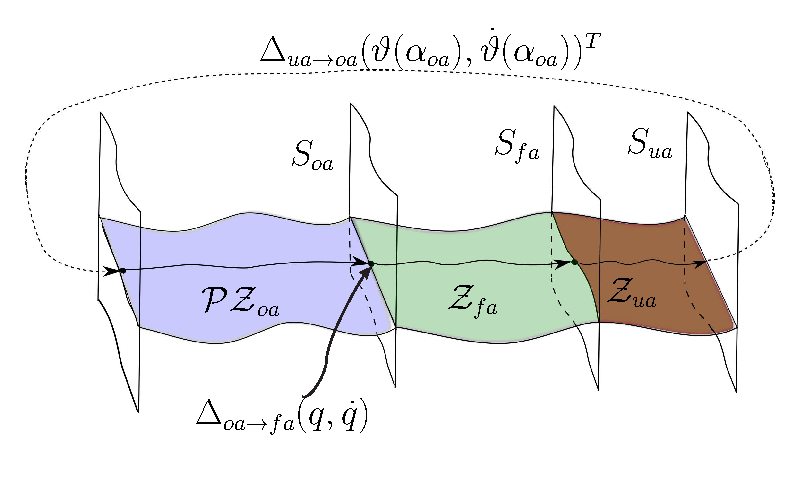
\includegraphics[scale=0.55]{figures/PZD_Surfaces_ICRA-crop.pdf}
% \hspace{-10mm}
\caption{Geometry of the close loop obtained using motion transitions.}
\label{fig:PZD_Surfaces}
% \vspace{50mm}
\end{figure}

\newsec{Human-Inspired Optimization.}
This section presents an optimization that yields controller parameters defining outputs that yield periodic, 3-domain walking. The key objective of the optimization is to find controller parameters defining referrence trajectories for each domain that minimize the least squares fit of these outputs to human walking data corresponding to the same outputs (see \cite{ZYA2012,YPA12} for the mathematical representation of this objective function).
%  From a subjects walking data, discrete times $t^{H}[k]$ and discrete values for the human output data, $y^{H}_{i,v}[k]$, for $i \in O_{v}$ where $O_{v}$ are indexing sets for the outputs in each domain $v \in V$. For clarity, the final discrete point in each domain will be denoted as $k_{v}$. For example, the last discrete time for the fully actuated domain will be referred to as $t[k_{fa}]$. With this in mind, the objective function for the human 
% inspired optimization is expressed mathematically as,
% \begin{align}
% \label{eq:cost}
% \hspace{-6mm} \mathrm{Cost_{HD}}(\alpha_{v}) = 
%  \sum\limits_{i \in O_{oa}}\sum\limits_{k = 1}^{k_{oa}}(y^{H}_{i}[k] - y^{d}_{oa,i}(t^{H}[k],\alpha_{oa,i}))^{2} \\ + 
%  \sum\limits_{j \in O_{fa}}\sum\limits_{k = k_{oa}}^{k_{fa}}(y^{H}_{j}[k] - y^{d}_{fa,j}(t^{H}[k],\alpha_{fa,j}))^{2} \hspace{-3mm} \nonumber \\ +
%  \sum\limits_{m \in O_{ua}}\sum\limits_{k = k_{fa}}^{k_{ua}}(y^{H}_{m}[k] - y^{d}_{ua,m}(t^{H}[k],\alpha_{ua,m}))^{2} \hspace{-6mm} \nonumber 
% \end{align}
% Minimizing this cost means finding controller parameters that are as close to the human data as possible thus resulting in humanlike locomotion.

\newsec{Force Based Constraints.} To compute force based constraints, the contact forces and moments at each contact point are computed using standard methods (see \cite{GCAS10}). The three contact conditions encountered in the 3 domain walking considered include: $c_{oa} = \{sh, nst\}$, $c_{fa} = \{st, sh\}$, and $c_{ua} = st$. Furthermore, a wrench containing contact forces and moments will exist for each point in contact, i.e. $F_{v,i} = (F^{x}_{v,i},F^{z}_{v,i},M^{y}_{v,i})$ for $i \in c_{v}$. A constraint is needed to ensure the vertical component of the contact force for each contact in each domain is greater than or equal to zero,
\begin{align}
min(F^{z}_{v,i}) \geq 0 \tag{C1}
\end{align}
Additionally, in order to prevent the feet from slipping, the following constraint must be satisfied:
\begin{align}
|F^{x}_{v,i}| < \frac{\mu}{\sqrt{2}} F^{z}_{v,i} \hspace{-3mm} \tag{C2-C6}
\end{align}
where $\mu$ is the friction coefficient of the walking surface. Also note that there will be a friction constraint 
for each contact point in each domains, leading to five friction constraints in total.

\newsec{Zero Dynamics Constraints.} The partial hybrid zero dynamics surface defined in \eqref{PZD} is defined for the continuous dynamics only, meaning any disturbances will lead to the system being thrown from this surface. It is for this that constraints are needed to ensure the zero dynamics surfaces are invariant to the 
impacts. To construct this constraint it is first necessary to define the \emph{full zero dynamics surface},
\begin{align}
\mathcal{Z}_{v} = \{(q,\dot{q}) \in Q : y_{v}(q) = \mathbf{0}, \dot{y}_{v}(q,\dot{q}) = \mathbf{0}\}
\end{align}
where $y_{v}(q)$ contains all relative degree one and/or two outputs in the domain $v$. With this, 
a constraint can be formulated to ensure the transition from full actuation to over actuation is 
invariant to the impact at heel strike. This constraint is expressed mathematically as,
\begin{align}
\Delta_{ua \rightarrow oa}(S_{ua} \cap \mathcal{Z}_{ua}) \subset \mathcal{PZ}_{oa} \tag{C7}
\end{align}
where $\Delta_{ua \rightarrow oa}$ represents the application of the impact map.

\newsec{Optimization Formulation.} With the controllers and constraints defined, the final form of the human inspired, 3-domain optimization becomes,
\begin{align}
\label{eq:OptimizationFinal}
 (\alpha^{*}_{v},d^{*}_{fa},d ^{*}_{ua}) =  \underset{\alpha_{oa},d_{fa},d_{ua}\in \mathbb{R}^{27}}{argmin}  \mathrm{Cost_{HD}}(\alpha_{v}) \\ \vspace{1mm}
 s.t. \hspace{3mm} (C1,C2,...,C7) \hspace{3mm} \nonumber
\end{align}
It is important to recall that $\alpha_{fa}$ and $\alpha_{ua}$ are solved for in closed form within the optimization 
using motion transitions, thus initial guesses for these parameters are not needed.
\begin{comment}
 These are the conditions needed to solve for controller parameters $\alpha$ corresponding to a motion transition from $(\q^{\sore}, \dq^{\sore})$ to  $(\q^{\tare}, \dq^{\tare})$:
\begin{align}
\label{eq:transitionsource}
  y^d_{2,{\tare}}(\timeparameterization_{\tare}(\q^{\sore}),\paramtransition_i) &= y^d_{2,{\sore}}(\timeparameterization_{\sore}(\q^{\sore}),\param_{\sore,i}) \nonumber\\
 {\dot y}^d_{2,{\tare}}(\timeparameterization_{\tare}(\q^{\sore}),\paramtransition_i) &={\dot y}^d_{2,{\sore}}(\timeparameterization_{\sore}(\q^{\sore}),\param_{\sore,i})\nonumber\\
 y^d_{2,{\tare}}(\timeparameterization_{\tare}(\q^{\tare}),\paramtransition_i) &= y^d_{2,{\tare}}(\timeparameterization_{\tare}(\q^{\tare}),\param_{\tare,i}) \nonumber\\
 {\dot y}^d_{2,{\tare}}(\timeparameterization_{\tare}(\q^{\tare}),\paramtransition_i) &= {\dot y}^d_{2,{\tare}}(\timeparameterization_{\tare}(\q^{\tare}),\param_{\tare,i}) 
\end{align}
for all $i \in \OutputSet_{\tare}$. 
\begin{myexample}
In this work, we construct two motion transitions $\alpha_{fa}$ and $\alpha_{ua}$. Naturally, the first transition,  $\alpha_{fa}$,  occurs at the first \textit{transition point}, $\beta_1$, i.e. when $ \timeparameterization_{\param_{oa}}(\q) = \beta_1$. The first motion transition connects $\resetmap_{oa \to fa} ( \guard_{oa \to fa} \cap \PartialZeroDynamics_{\param_{oa}} )$ to $(\thetaalpha, \thetaalphadot)$.  Likewise, the second transition , $\alpha_{ua}$, occurs at the second transition point, $\beta_2$, i.e. when $ \timeparameterization_{\param_{fa}}(\q) = \beta_2$. The second motion transition connects $\resetmap_{fa \to ua} ( \guard_{fa \to ua} \cap \PartialZeroDynamics_{\param_{fa}} )$ with $(\thetaalpha, \thetaalphadot)$.
\end{myexample}

\begin{comment}
%HERE IS AN ALTERNATE EXPRESSION FOR A MOTION TRANSITIONS (FAIL)
%\begin{mydefinition}
%Controller parameters $\alpha$ of the extended canonical walking function are said to form a \textit{Motion Transition} from $x_1 = (\q_1^T,\dq_1^T)^T$ to  $x_2 = (\q_2^T,\dq_2^T)^T $ REF if
%\begin{align}
%\exists \alpha \st &  \:\: \nonumber \\
% (\q_1^T,\dq_1^T)^T  &\in \PartialZeroDynamics_{\alpha} \\
% (\q_2^T,\dq_2^T)^T  &\in \PartialZeroDynamics_{\alpha}
%\end{align}
%\end{mydefinition}


%
%In particular, the velocities, $\thetaalphadot$ are obtained through
%\begin{align}
%\label{eq:inverse_dot}
%\thetaalphadot = \left[ \begin{array}{c} \indexbyvertex{\dyonedq} \\ \indexbyvertex{\dytwodq} \end{array} \right]^{-1} \left( \begin{array}{c} \vhip \\ \zm \end{array} \right).
%\end{align}




%\begin{align}
%\qreconstruction(\xi_{1,\vertex}) &= \left[ \begin{array}{c} \indexbyvertex{\dyonedq} \\ \indexbyvertex{\dytwodq} \end{array} \right]^{-1} \left( \begin{array}{c} \xi_{1,\vertex} \\ \ydtwo (\xi_{1,\vertex}) \end{array} \right)\\
%\dqreconstruction(\xi_{1,\vertex}) &= \left[ \begin{array}{c} \indexbyvertex{\dyonedq} \\ \indexbyvertex{\dytwodq} \end{array} \right]^{-1} \left( \begin{array}{c} 1 \\ \frac{\partial \ydtwo (\xi_{1,\vertex})}{\partial \xi_{1,\vertex}} \end{array} \right)
%\end{align}



%\newsec{Optimization Cost.}
%The objective function of this optimization is a least squares fit of controller outputs to corresponding outputs computed on human locomotion data, over all three domains. The controller parameters for the full actuation, $\indexbyfullactuation{\param}$, and the under actuation, $\indexbyunderactuation{\param}$, domains are obtained through motion transitions, specifically \eqref{eq:transitionsource} and \eqref{eq:transitiontarget}. The human data, with discrete times $t^H[k]$ and values for outputs, $y^H_i[k]$, is indexed by a set $K$, where $k \in \{1, \ldots, K\}$ represents indices for discrete data points, and $t^H[k] < t^H[k+1] \forall k \in K$. Let $K_{\beta_1}$ denote the time corresponding to a transition from $oa \to fa$ and $K_{\beta_2}$ denote the time corresponding to a transition from $fa \to ua$. For each relative degree two output, $i \in \OutputSet_v$ for a given domain, $\vertex \in \VertexSet$, the value of the output is denoted $y^d_i(t^H[k],\param_{v,i})$  . The total cost is the sum of the costs of each domain, which can be stated as follows
%\begin{align}
%\nonumber
%\costoa(\indexbydoublesupport{\param} ) =  \sum_{k = 1}^{K_{\beta_1}} \sum_{i \in \OutputSet_{oa}} \left( y^H_i[k] - y^d_i(t^H[k],\param_{oa,i}) \right)^2
%\end{align}
%\begin{align}
%\nonumber
%\costfa(\indexbydoublesupport{\param} ) =  \sum_{k = K_{\beta_1}}^{K_{\beta_2}} \sum_{i \in \OutputSet_{fa}} \left( y^H_i[k] - y^d_i(t^H[k],\alpha_{(fa,i)}(\param_{oa}) \right)^2
%\end{align}
%\begin{align}
%\nonumber
%\costua(\indexbydoublesupport{\param} ) =  \sum_{k = K_{\beta_2}}^{K} \sum_{i \in \OutputSet_{ua}} \left( y^H_i[k] - y^d_i(t^H[k],\alpha_{(ua,i)}(\param_{oa})  \right)^2
%\end{align}
%\begin{align}
%\label{eq:HDBC}
%\HDBC(\indexbydoublesupport{\param} ) =  \costoa(\indexbydoublesupport{\param} ) + \costfa(\indexbydoublesupport{\param} )+ \costua(\indexbydoublesupport{\param} )
%\end{align}
%which quantifies the similarity between the human and the robot outputs.



\newsec{Optimization Problem Statement.} The goal of \textit{human-inspired PHZD optimization} is to find parameters $\indexbydoublesupport{\param^*}$ that solve the following constrained optimization problem:
\begin{align}
\label{eq:PHZDopt}
\tag{HIO}
(\indexbydoublesupport{\param}^*, \beta^*) = \underset{(\indexbydoublesupport{\param}, \beta)  \in \Reals^{21} \times \Reals^{2} }{\operatorname{argmin}} &  \:\: \HDBC(\indexbydoublesupport{\param} )  \\
%\tag{C}
\st &  \:\: \nonumber \\
\label{eq:C1}
\tag{C1}
\resetmap_{fa \to oa} ( \guard_{fa \to oa} \cap \PartialZeroDynamics_{\alpha_{fa}(\param_{oa}, \beta)} ) &\subset \PartialZeroDynamics_{\param_{oa}} \\
\label{eq:C2}
\tag{C2}
\resetmap_{oa \to ua} ( \guard_{oa \to ua} \cap \PartialZeroDynamics_{\param_{oa}} ) &\subset \PartialZeroDynamics_{\alpha_{ua}(\param_{oa}, \beta)}  \\
\label{eq:C3}
\tag{C3}
\resetmap_{ua \to fa} ( \guard_{ua \to fa} \cap \PartialZeroDynamics_{\alpha_{ua}(\param_{oa}, \beta)} ) &\subset \PartialZeroDynamics_{\alpha_{fa}(\param_{oa}, \beta)} \\
\label{eq:C4}
\tag{C4}
(\qreconstruction (\beta_1), \dqreconstruction (\beta_1)) &\in \guard_{oa \to fa} \\
\label{eq:C5}
\tag{C5}
(\qreconstruction (\beta_2), \dqreconstruction (\beta_2)) &\in \guard_{fa \to ua} \\
\label{eq:C6}
\tag{C6}
\indexbydoublesupport{\ConstraintMatrix}(\qreconstruction (\xi_{1,oa}),\dqreconstruction (\xi_{1,oa}), \indexbydoublesupport{\control}) &\geq 0 \\
\label{eq:C7}
\tag{C7}
\indexbyfullactuation{\ConstraintMatrix}(\qreconstruction (\xi_{1,fa}),\dqreconstruction (\xi_{1,fa}), \indexbyfullactuation{\control}) &\geq 0 \\
\label{eq:C8}
\tag{C8}
\indexbyunderactuation{\ConstraintMatrix}(\qreconstruction (\xi_{1,ua}),\dqreconstruction (\xi_{1,ua}), \indexbyunderactuation{\control}) &\geq 0
\end{align}
where $\HDBC(\param_{oa})$ is essentially the same cost as the original human data based cost given in EQREF.; where here, the contribution to the cost in each domain is the least squares fit of human data to the desired values of each controller output. Note that the motion transitions, $\alpha_{fa}$ and $\alpha_{ua}$, are functions of both $\alpha$ and $\beta$ because 

\begin{algorithm}
\caption{Algorithm for obtaining controller parameters for a three-domain locomotion gait.}
%The optimization procedure follows:
\begin{itemize}[\setlabelwidth{Step 1}]
\item[Step 1)] Initialize values for the controller parameters, $\param_{oa}$, and the domain transition points, $\beta$.
\item[Step 2)] Solve the inverse kinematics problem, yielding $(\thetaalpha, \thetaalphadot)$-- the initial condition to the double support domain on the partial hybrid zero dynamics surface.
\item[Step 3)] Compute the state reconstruction for the double support domain and use this reconstruction to compute inequality constraints \eqref{eq:C6} on the domain of admissibility $\domain_{oa}$ for double support.
\item[Step 4)] Compute the state reconstruction at the first transition point, $\xi_{1,oa} = \beta_1$, and use this point to compute equality \eqref{eq:C4} constraints on the guard from double support to full actuation, $\guard_{oa \to fa}$.
\item[Step 5)] Compute parameters for the full actuation domain, $\alpha_{fa}$, that construct a motion transition EQREF from $(\qreconstruction (\beta_1),\dqreconstruction (\beta_1),\param_{fa}) \to (\thetaalpha, \thetaalphadot)$ .
\item[Step 6)] Compute the state reconstruction for the full actuation domain and use this reconstruction to compute inequality constraints \eqref{eq:C7} on the domain of admissibility $\domain_{fa}$ for full acutation.
\item[Step 7)] Compute the state reconstruction at the second transition point,  $\xi_{1,fa} = \beta_2$,  and use this point to compute equality \eqref{eq:C5} constraints on the guard from full actuation to under actuation, $\guard_{fa \to ua}$.
\item[Step 8)] Compute parameters for the under actuation domain, $\tilde{\alpha}_{ua}$, that construct a motion transition EQREF from $(\qreconstruction (\beta_2),\dqreconstruction (\beta_2),\param_{ua}) \to (\thetaalpha, \thetaalphadot)$.
\item[Step 9)] Integrate through the underactuated domain to compute inequality constraints \eqref{eq:C8} on the domain of admissibility $\domain_{ua}$ for under actuation.
\item[Step 10)] Compute $\HDBC(\param_{oa})$.
\item[Step 11)] Iterate the nonlinear constrained optimization problem one step, \ref{eq:PHZDopt}, to obtain values for $\param_{oa}$ and $\beta$.
\item[Step 12)] Repeat the iteration until local minimum reached, yielding optimal controller parameters, $\param_{oa}^*$, and domain transition points, $\beta^*$.
\end{itemize}
\end{algorithm}
\end{comment}

\section{\uppercase{Quadratic Programs}}
\label{sec:QP}

The chief obstacle in designing controllers for multi-domain, multi-contact locomotion lies in the constantly changing degree of actuation. Over actuated domains provide a unique issue from a controls perspective, namely that there are not a unique set of actuator torques to meet a control objective. In the case of I/O Linearization, this results in singularities in the decoupling matrix. This section presents an online QP to select optimal actuator torques to achieve convergence.

Since torque saturation is a common issue in bipedal robots, the desire is to pose a QP that will meet the control objective while being optimal with respect to the amount of actuator torque requested. First recall that for $v \in \{V_{oa},V_{fa}\}$,  the control law for these domains is given in Equation \eqref{eqn:uv}. This can be rewritten in the following form,
\begin{align}
\hspace{-3mm}-\indexbyvertex{\decouplingmatrix}(\q,\dq)\indexbyvertex{\control^{(\param_{v},\controlgain)}}(\q,\dq)& = \left( \left[ \begin{array}{c} 0 \\ L_{f_v}L_{f_v}\ytwo(\q, \dq) \end{array} \right]\right. \tag{QPC1} \\ 
& \hspace{-20mm}+ \left.\left[ \begin{array}{c} L_{f_v}\yone(\q, \dq) \\ 2 \controlgain L_{f_v}\ytwo(\q, \dq) \end{array} \right] + \left[ \begin{array}{c} \controlgain \yone(\q,\dq) \\ \controlgain^2 \ytwo(\q) \end{array} \right] \right) \nonumber
\end{align}
in which it can be posed as a constraint to a QP, resulting in the following control law:
\begin{align}
  u^{*}_{v} = \underset{u_{v} \in \mathbb{R}^{9}}{\mathrm{argmin}} \hspace{3mm} u^{T}_{v}W_{v} u_{v} \hspace{0mm} \\
 s.t. \hspace{5mm} \mathrm{(QPC1)} \hspace{-10mm} \nonumber
\end{align}
where $W_{v}$ is a $9 \times 9$ torque distribution matrix that can be used to distribute the torques to allow certain actuators to do more of the work than others if necessary based on actuator capabilities. For the robot model being used here, the torque distribution matrix takes the form,
\begin{align}
\label{eq:torquedist}
 W_{v} = 
 \begin{bmatrix}
  \mathbf{0}_{3 \times 3} & \mathbf{0}_{3 \times 6} \\
  \mathbf{0}_{6 \times 3} & (\omega_{v})_{m_{r} \times m_{r}}
 \end{bmatrix}
\end{align}
where $m_{r}$ the number of actuators on the robot, and $\omega_{v}$ is a $m_{r} \times m_{r}$ diagonal matrix describing in which the elements on the diagonal reflect the desired torque distribution. If, for example, each actuator is to be weighted equally, $\omega_{v}$ is the identity matrix. Similarly, the same can be done for $v \in V_{ua}$ where the original control law is rewritten as,
\begin{align}
-\indexbyvertex{\decouplingmatrix}(\q,\dq) \indexbyvertex{\control^{(\param_{v},\controlgain)}}(\q,\dq) = & \left( L_{f_v}L_{f_v}\ytwo(\q,\dq) + \right. \tag{QPC2} \\
 & \hspace{-10mm} \left. 2 \controlgain L_{f_v}\ytwo(\q,\dq) + \controlgain^2 \ytwo(\q)\right) \nonumber
\end{align}
With this, the resulting control law for $v \in V_{ua}$ becomes,
\begin{align}
 u^{*}_{ua} = \underset{u_{ua} \in \mathbb{R}^{9}}{\mathrm{argmin}} \hspace{3mm} u^{T}_{ua}W_{ua} u_{ua} \hspace{0mm} \\
  s.t. \hspace{5mm} \mathrm{(QPC2)} \hspace{-10mm} \nonumber
\end{align}
These QP's not only allow for the distribution of torque, they also do not require the inversion of the decoupling matrix, meaning that during over actuation the QP can minimize torque while meeting the convergence objectives.


\section{Simulation Results}
\label{sec:simresults}

This section presents a simulation example showing how the optimization algorithm of Section \ref{sec:optimization} was used to produce a multi-domain walking gait for the planar biped AMBER 2, a planar robot that was designed and partially machined within AMBER lab at Texas A\&M University. AMBER 2 is a seven link robot supported by a light weight, carbon fiber boom that restricts motion to the saggital plane. The boom is counter weighted so as to not introduce mass to the robot; however, there is an inertial load introduced to the torso link that is negligable due to the low friction bearings used in the construction of the boom as well as a long moment arm ($\sim$ 8ft) separating the robot from the center of rotation of the boom.
\begin{figure}
\centering
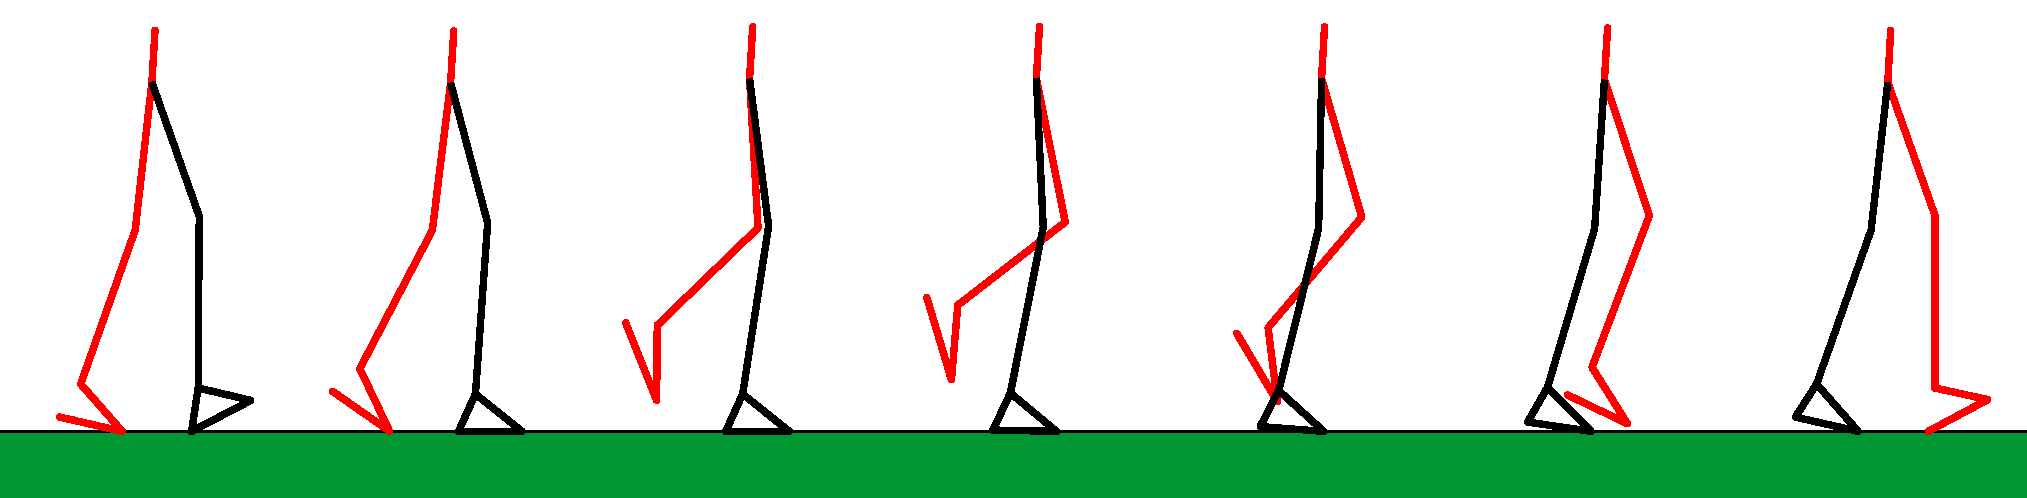
\includegraphics[scale=0.26]{figures/Tiles.pdf}
\caption{Gait tiles for a 3 domain walking gait.}
\label{fig:Tiles}
\end{figure} 
%The mass and length parameters of AMBER 2 are shown in Table \ref{table:params} with variable conventions as defined in Fig. \ref{fig:robotCoords}.
The optimization of Section \ref{sec:optimization} was implemented using MATLAB'S FMINCON function and the interior-point algorithm.
% \begin{table}[H]
% \caption{AMBER 2.0 Mass \& Length Parameters}
% \centering
% \begin{tabular}{c c c c}
% \hline\hline
% Link & Mass(g) & Length(mm) & Width(mm) \\ [0.5ex]
% \hline
% Foot & 204.42 & 177.8 & 47.63 \\
% Calf & 1119.43 & 343.13 & 50.8 \\
% Thigh & 1172.57 & 298.45 & 50.8 \\
% Torso & 2154.79 & 104.01 & 285.75 \\ [1ex]
% \hline	
% \end{tabular}
% \label{table:params}
% \end{table}
For the underactuated phase, the integration algorithm ODE45
was used to integrate the dynamics forward in time.  In both the double support and fully actuated phases, the solution at each timestep was found in closed-form using the reconstruction algorithm discussed in Section \ref{sec:reconstruction}.
\begin{figure}[t!]
\centering
\begin{subfigure}{0.001\textwidth}
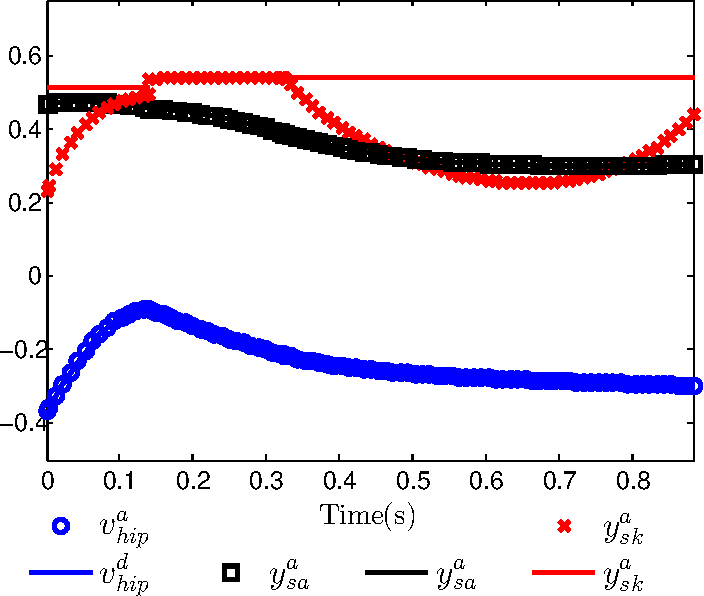
\includegraphics[width=42mm]{figures/YaVsYd1-crop.pdf}
\vspace{-42mm}
\end{subfigure}
\begin{subfigure}{0.75\textwidth}
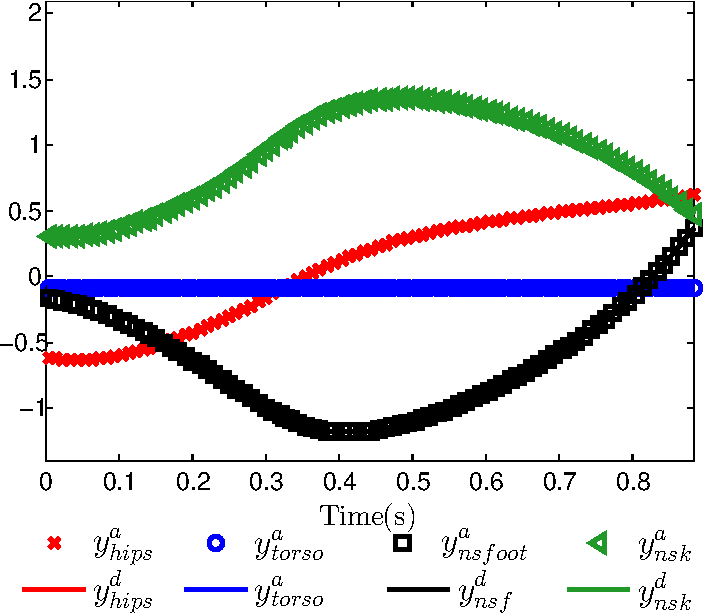
\includegraphics[width=42mm]{figures/YaVsYd2-crop.pdf}

\end{subfigure}
\caption{Actual and desired outputs over one step for a 3 domain walking gait.}
\label{fig:Outputs}
\end{figure}
The results of the optimization are shown in Fig. \ref{fig:Tiles}, where the 3-domain walking gait is plotted as a series of tiles. 
An animation is available at [\url{http://www.youtube.com/watch?v=OY-QsaIglQY}].  The gait shown here has an average velocity of 0.42 m/s, with a step length
of 0.373 m (58\% of leg length) and a period of $T = 0.88$ sec. The step time can be further broken down, with 0.139 s (16\%) in double 
support / overactuation, 0.19 s (21\%) in full actuation, and 0.56 s (63\%) in underaction. The actual and desired outputs for the gait are shown in Fig. \ref{fig:Outputs}.

The joint torques over one step with I/O Linearization and the QP are compared in Fig. \ref{fig:Torques}. Notice that for simple I/O Linearization, the torque at the nonstance ankle is identically zero for 
the domain of over actuation. This is due to the configuration of the robot only containing 5 independent degrees of freedom. With the QP, however, torques for all six actuators can be specified and, additionally, there is a decrease in the maximum required torque($\sim$33 Nm for I/O Linearization and 24 Nm for QP).
%
\begin{figure}[t!]
\centering
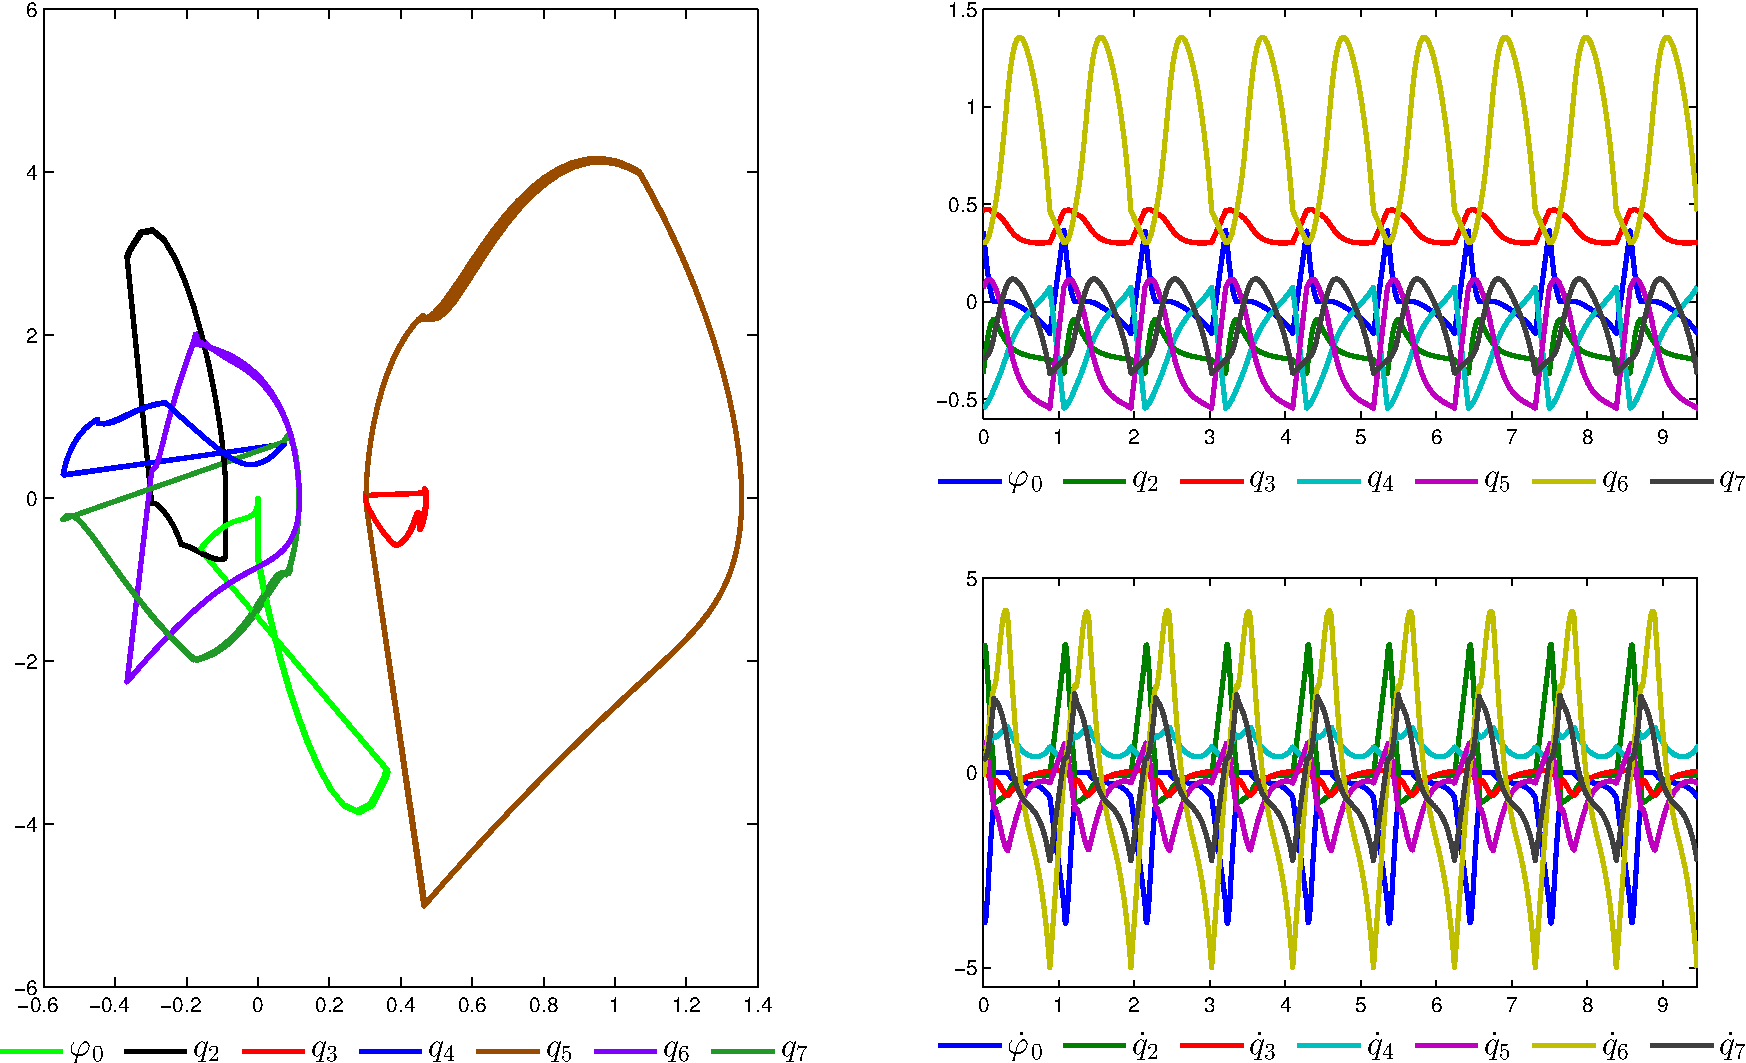
\includegraphics[scale=0.3]{figures/subplot_orbit-crop.pdf}
% \hspace{-10mm}
\caption{Phase plot (left) for 9 steps of a 3 domain walking gait showing the periodicity of the gait and joint angles (top right) and velocities (bottom right).}
\label{fig:subplot_orbit}
% \vspace{50mm}
\end{figure}
% 
\begin{figure}[t!]
\centering
\begin{subfigure}{0.75\textwidth}
\hspace{-5mm}
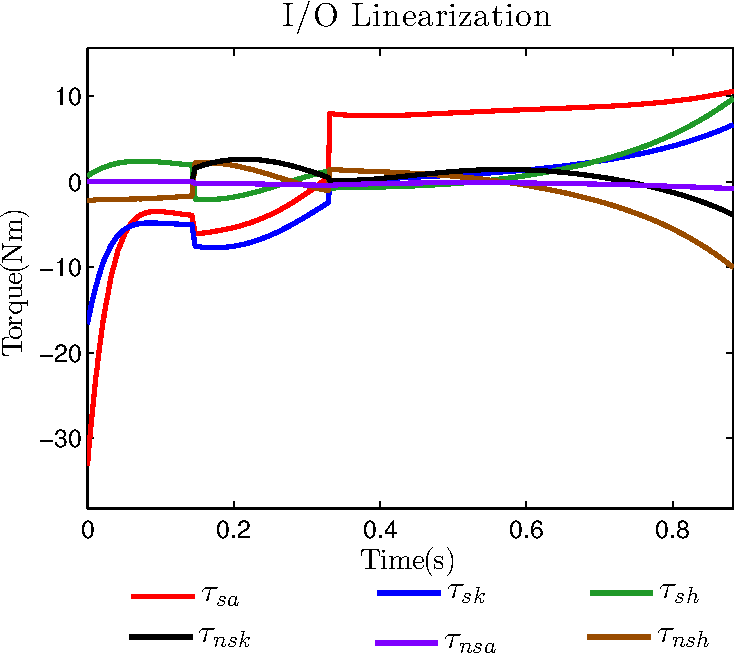
\includegraphics[width=44mm]{figures/TORK_IO-crop.pdf}
\end{subfigure}
\begin{subfigure}{0.001\textwidth}
\vspace{-39mm}
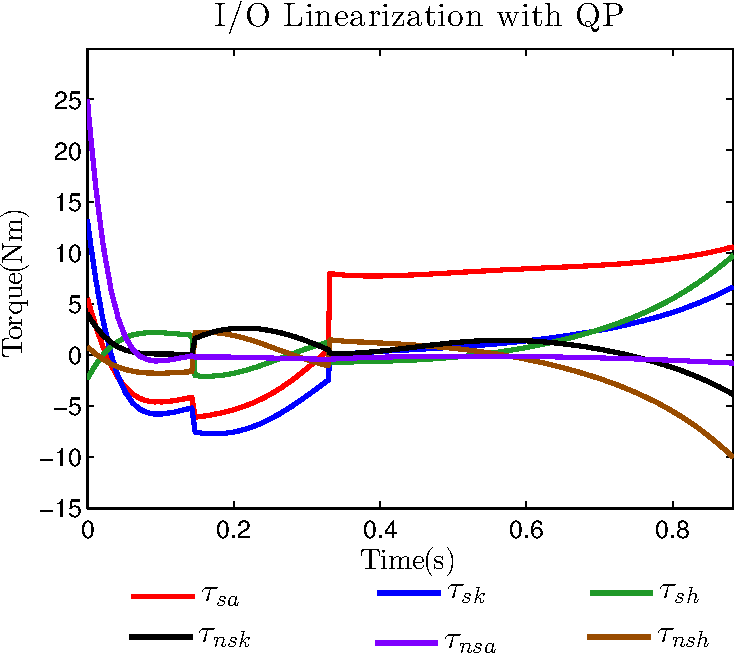
\includegraphics[width=44mm]{figures/TORK_QP-crop.pdf}
\end{subfigure}
\caption[Plots comparing joint torques from I/O Linearization and the QP.]{Joint torques over one step using I/O Linearization(left) and the quadratic program(right).}
\label{fig:Torques}
%\vspace{15cm}
\end{figure}


\section{Conclusion}

The objective of this paper has been to present a novel method with which to design multi-domain walking gaits. It began with the introduction of multi-domain hybrid systems followed by the introduction of the floating base model. The principle contribution lies, however, in the multi-domain human inspired optimization. Using the human inspired optimization, walking gaits can be designed and shaped by altering constraints. The human-like walking presented here was achieved using I/O Linearization, but with the use of a QP a single control law to be used for domains with differing degrees of actuation. The methods described here have been recently realized on AMBER 2 to achieve robust, multi-domain locomotion \cite{url:AMBER2_MultiContact}.

\bibliographystyle{abbrv}
\bibliography{bibdata}

\end{document}
